% Options for packages loaded elsewhere
\PassOptionsToPackage{unicode}{hyperref}
\PassOptionsToPackage{hyphens}{url}
%
\documentclass[
]{article}
\usepackage{amsmath,amssymb}
\usepackage{lmodern}
\usepackage{ifxetex,ifluatex}
\ifnum 0\ifxetex 1\fi\ifluatex 1\fi=0 % if pdftex
  \usepackage[T1]{fontenc}
  \usepackage[utf8]{inputenc}
  \usepackage{textcomp} % provide euro and other symbols
\else % if luatex or xetex
  \usepackage{unicode-math}
  \defaultfontfeatures{Scale=MatchLowercase}
  \defaultfontfeatures[\rmfamily]{Ligatures=TeX,Scale=1}
\fi
% Use upquote if available, for straight quotes in verbatim environments
\IfFileExists{upquote.sty}{\usepackage{upquote}}{}
\IfFileExists{microtype.sty}{% use microtype if available
  \usepackage[]{microtype}
  \UseMicrotypeSet[protrusion]{basicmath} % disable protrusion for tt fonts
}{}
\makeatletter
\@ifundefined{KOMAClassName}{% if non-KOMA class
  \IfFileExists{parskip.sty}{%
    \usepackage{parskip}
  }{% else
    \setlength{\parindent}{0pt}
    \setlength{\parskip}{6pt plus 2pt minus 1pt}}
}{% if KOMA class
  \KOMAoptions{parskip=half}}
\makeatother
\usepackage{xcolor}
\IfFileExists{xurl.sty}{\usepackage{xurl}}{} % add URL line breaks if available
\IfFileExists{bookmark.sty}{\usepackage{bookmark}}{\usepackage{hyperref}}
\hypersetup{
  pdftitle={Analysis of The Carpentries Long-Term Surveys},
  pdfauthor={François Michonneau; Kari L. Jordan},
  hidelinks,
  pdfcreator={LaTeX via pandoc}}
\urlstyle{same} % disable monospaced font for URLs
\usepackage[margin=1in]{geometry}
\usepackage{graphicx}
\makeatletter
\def\maxwidth{\ifdim\Gin@nat@width>\linewidth\linewidth\else\Gin@nat@width\fi}
\def\maxheight{\ifdim\Gin@nat@height>\textheight\textheight\else\Gin@nat@height\fi}
\makeatother
% Scale images if necessary, so that they will not overflow the page
% margins by default, and it is still possible to overwrite the defaults
% using explicit options in \includegraphics[width, height, ...]{}
\setkeys{Gin}{width=\maxwidth,height=\maxheight,keepaspectratio}
% Set default figure placement to htbp
\makeatletter
\def\fps@figure{htbp}
\makeatother
\setlength{\emergencystretch}{3em} % prevent overfull lines
\providecommand{\tightlist}{%
  \setlength{\itemsep}{0pt}\setlength{\parskip}{0pt}}
\setcounter{secnumdepth}{-\maxdimen} % remove section numbering
\usepackage{float}
\usepackage{array}
\usepackage{booktabs}
\usepackage[table]{xcolor}
\ifluatex
  \usepackage{selnolig}  % disable illegal ligatures
\fi

\title{Analysis of The Carpentries Long-Term Surveys}
\author{François Michonneau\footnote{\url{http://orcid.org/0000-0002-9092-966X}} \and Kari
L. Jordan\footnote{\url{https://orcid.org/0000-0003-4121-2432}}}
\date{June 29, 2021}

\begin{document}
\maketitle

{
\setcounter{tocdepth}{2}
\tableofcontents
}
In the fourth quarter of 2020 The Carpentries collected feedback from
community members who took a Carpentries workshop within six months.
Find more information about this data collection period
\href{https://carpentries.org/blog/2020/09/long-term-survey-is-now-open/}{on
our blog}. We are excited to release the results of our long-term
survey, and invite community members to use this data to champion The
Carpentries far and near.

We released
\href{https://datacarpentry.org/blog/2017/10/long-term-survey-results}{our
first long-term survey results} in October 2017. You can find
\href{https://github.com/carpentries/assessment/blob/master/learner-assessment/archives/2017/reports/longtermreport_October2017.pdf}{the
report} and
\href{https://github.com/carpentries/assessment/blob/master/learner-assessment/archives/2017/code/longtermreport_October2017.rmd}{its
source} in the
\href{https://github.com/carpentries/assessment/blob/master/learner-assessment/}{assessment
GitHub repository}.

We released our latest long-term survey results in April 2020. You can
find
\href{https://github.com/carpentries/assessment/blob/master/learner-assessment/reports/2020-01-long-term-report.pdf}{the
report} and
\href{https://github.com/carpentries/assessment/blob/master/learner-assessment/reports-src/2020-01-long-term-survey.Rmd}{its
source} in the
\href{https://github.com/carpentries/assessment/blob/master/learner-assessment/}{assessment
GitHub repository}.

The results included in this report only cover the data collected in
2020 (between September 28th, 2020 and November 1st, 2020). This report
includes the analysis of 263 responses but most questions are optional
and specific questions have less answers.

\hypertarget{respondents-career-stage}{%
\subsection{Respondents Career Stage}\label{respondents-career-stage}}

The majority of long-term survey respondents are graduate students.
``Other academic staff'' includes Librarians, Research Software
Engineers, IT Staff, and Government Research Staff.

\begin{verbatim}
## Warning: It is deprecated to specify `guide = FALSE` to remove a guide.
## Please use `guide = "none"` instead.
\end{verbatim}

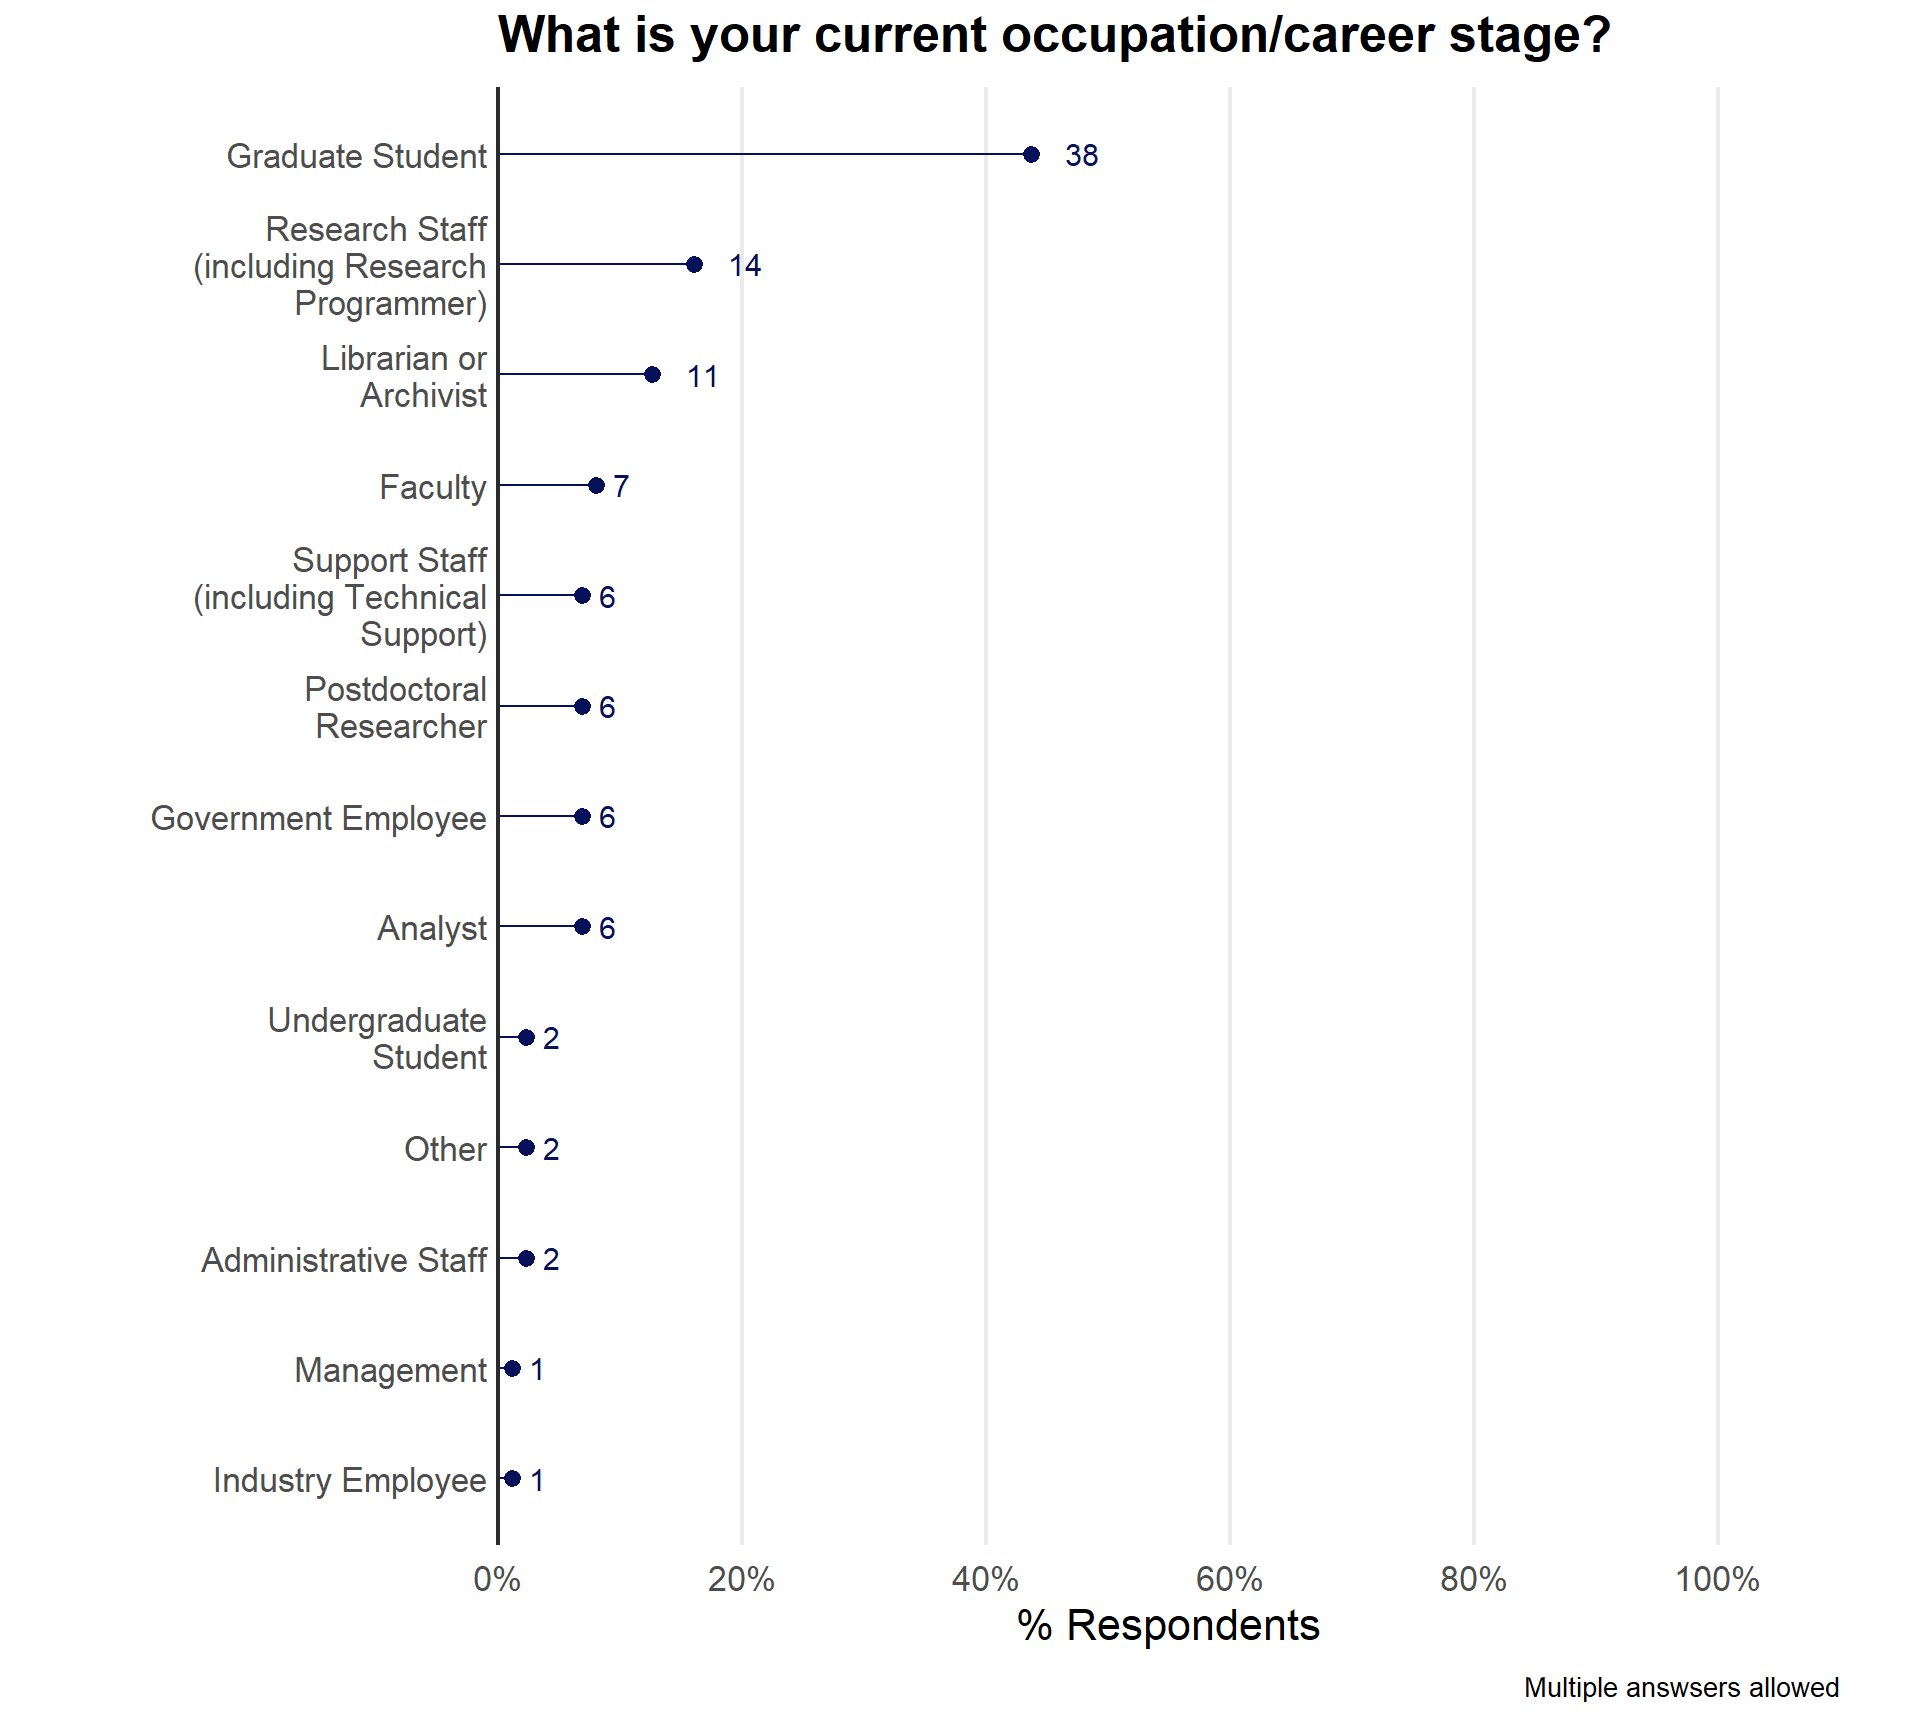
\includegraphics[width=\maxwidth]{../figures/2020-12-longterm-occupation-1}

\hypertarget{respondents-field-of-research-work-or-study}{%
\subsection{Respondents Field of Research, Work, or
Study}\label{respondents-field-of-research-work-or-study}}

The largest percentages of long-term survey respondents were from the
Life Sciences (19\%) followed by Library and Information Science (17\%).

\begin{verbatim}
## Warning: It is deprecated to specify `guide = FALSE` to remove a guide.
## Please use `guide = "none"` instead.
\end{verbatim}

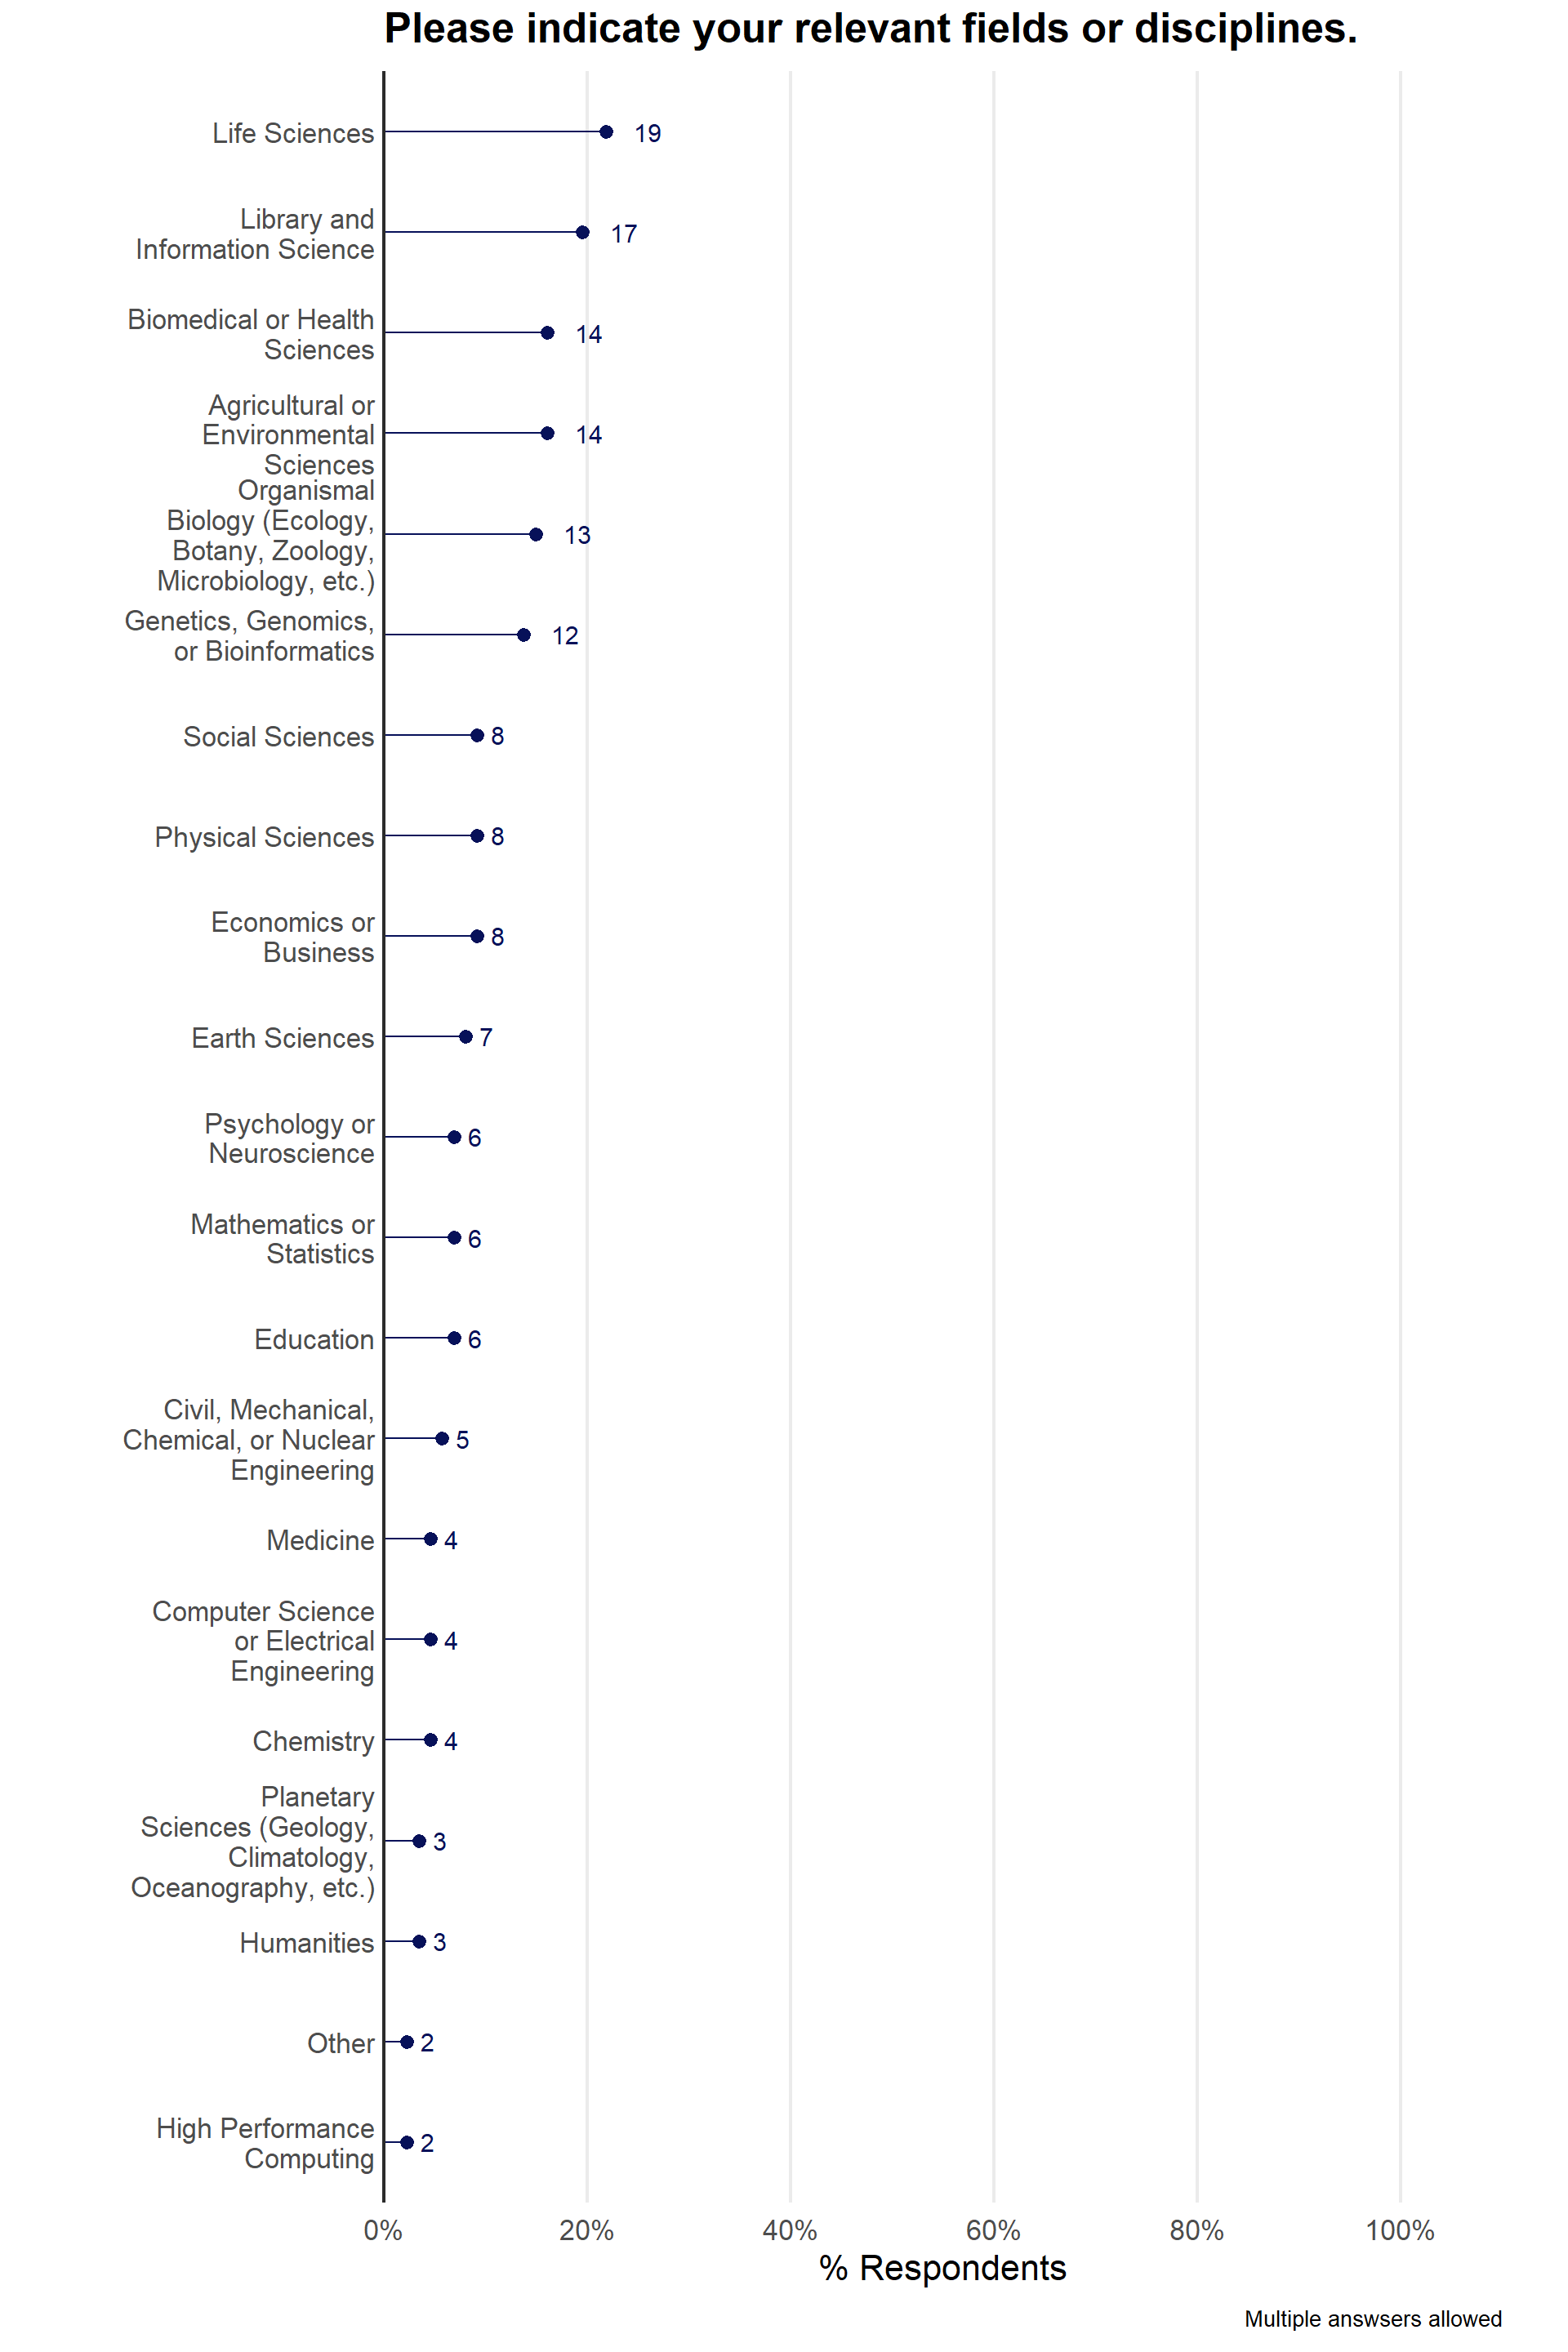
\includegraphics[width=\maxwidth]{../figures/2020-12-longterm-domain-1}

\hypertarget{number-of-carpentries-workshops-completed}{%
\subsection{Number of Carpentries Workshops
Completed}\label{number-of-carpentries-workshops-completed}}

The majority of long-term survey respondents have completed just one
Carpentries (Software, Data, or Library) workshop. The percentage of
those who have completed only one workshop is up from the previous year.

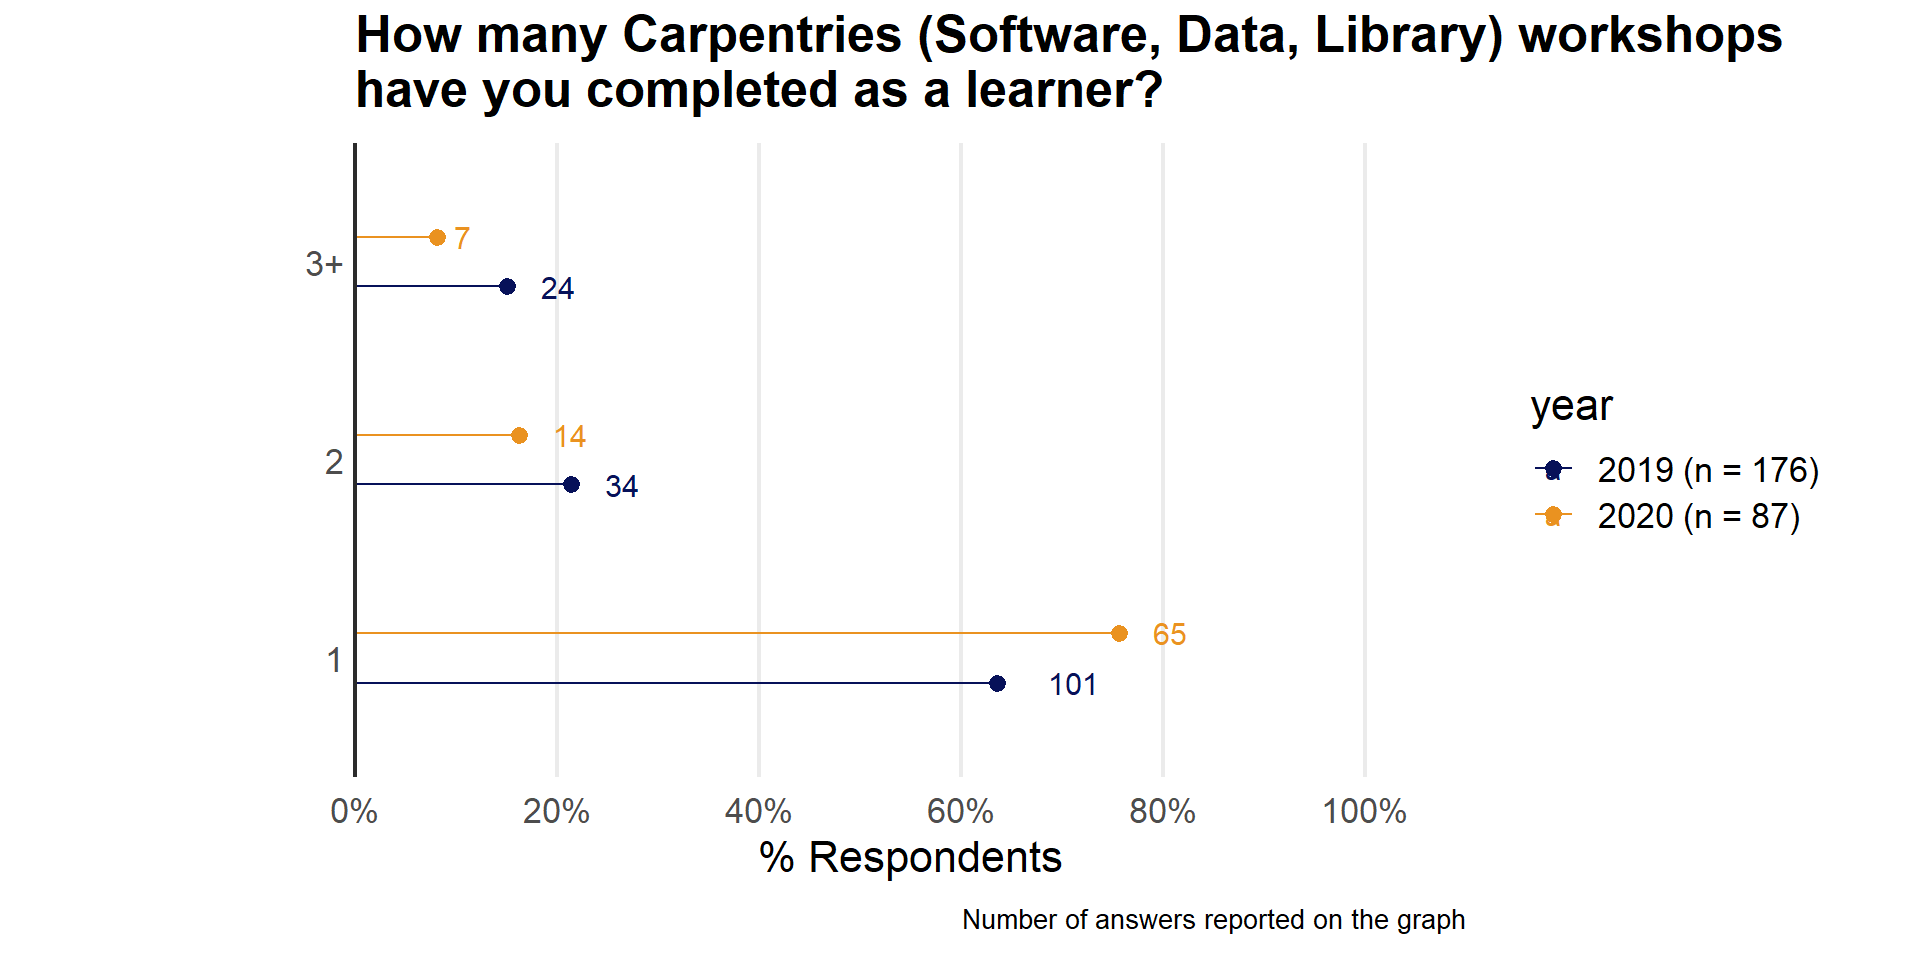
\includegraphics[width=\maxwidth]{../figures/2020-12-longterm-workshop_attended_amount-1}

\hypertarget{time-since-completing-a-carpentries-workshop}{%
\subsection{Time Since Completing a Carpentries
Workshop}\label{time-since-completing-a-carpentries-workshop}}

The majority of long-term survey respondents last completed a
Carpentries workshop between 0 and 6 months ago. In 2019, there was a
higher percentage of responses from those who had completed a workshop
more than a year ago.

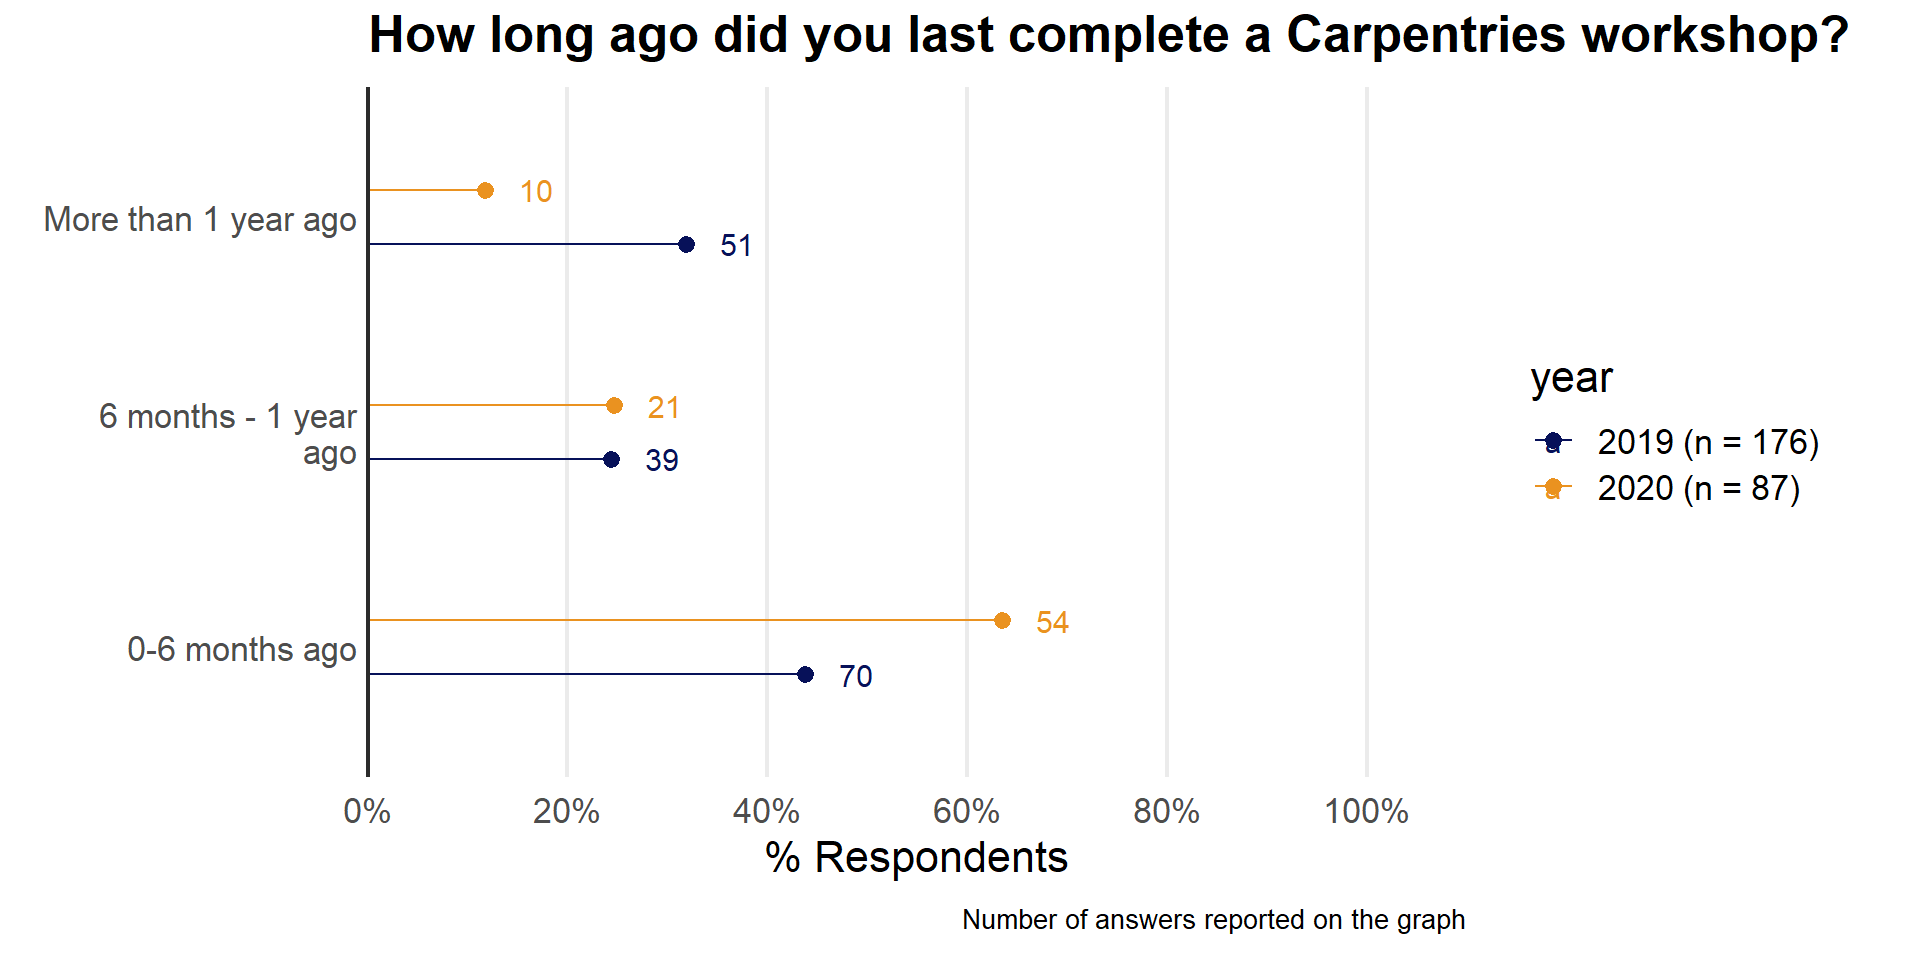
\includegraphics[width=\maxwidth]{../figures/2020-12-longterm-workshop_attended_age-1}

\hypertarget{last-carpentries-workshop-attended}{%
\subsection{Last Carpentries Workshop
Attended}\label{last-carpentries-workshop-attended}}

Long-term survey respondents were almost evenly split on whether their
last Carpentries workshop was a Data or Software Carpentry workshop with
Software Carpentry being slightly more common than Data Carpentry. A
much smaller percentage of respondents said their last Carpentries
workshop was a Library Carpentry workshop.

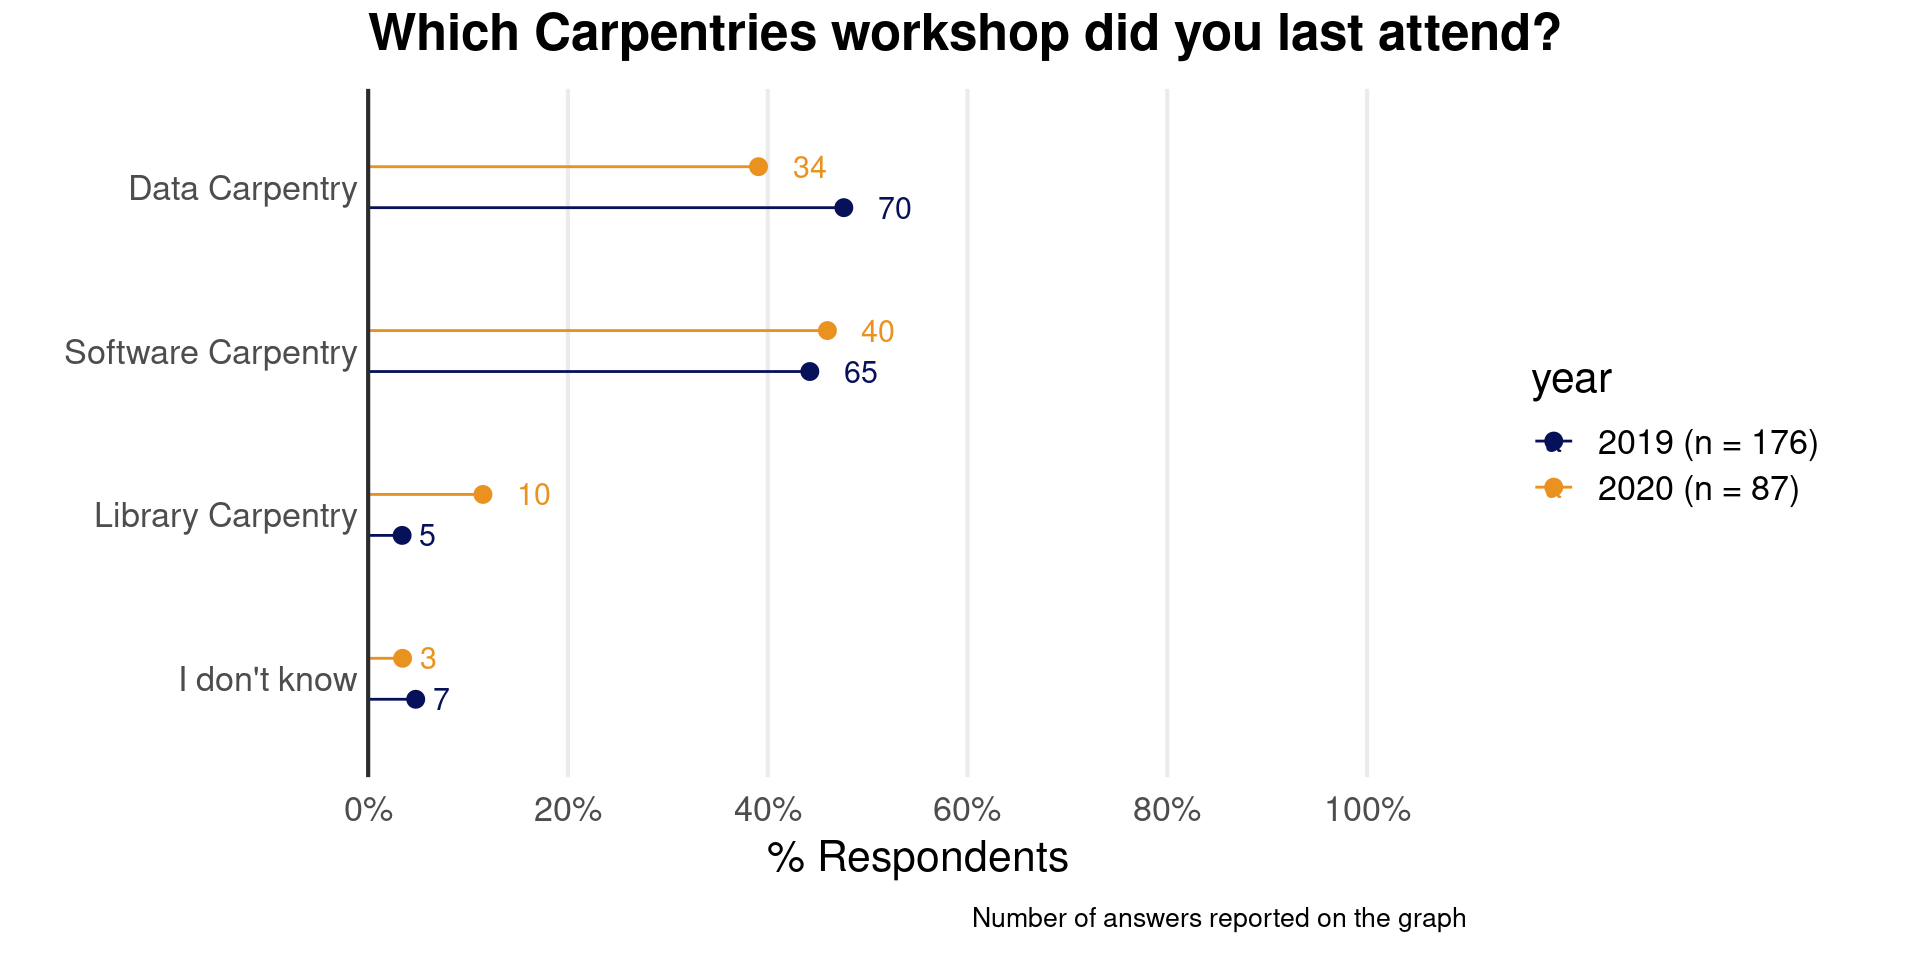
\includegraphics[width=\maxwidth]{../figures/2020-12-longterm-workshop_attended_type-1}

\hypertarget{content-covered-at-last-carpentries-workshop}{%
\subsection{Content Covered at Last Carpentries
Workshop}\label{content-covered-at-last-carpentries-workshop}}

In 2020, the most common content taught (as reported by long-term survey
respondents) was Git followed by the Unix Shell and Python. A much lower
percentage of respondents reported their workshop covered R compared
with 2019.

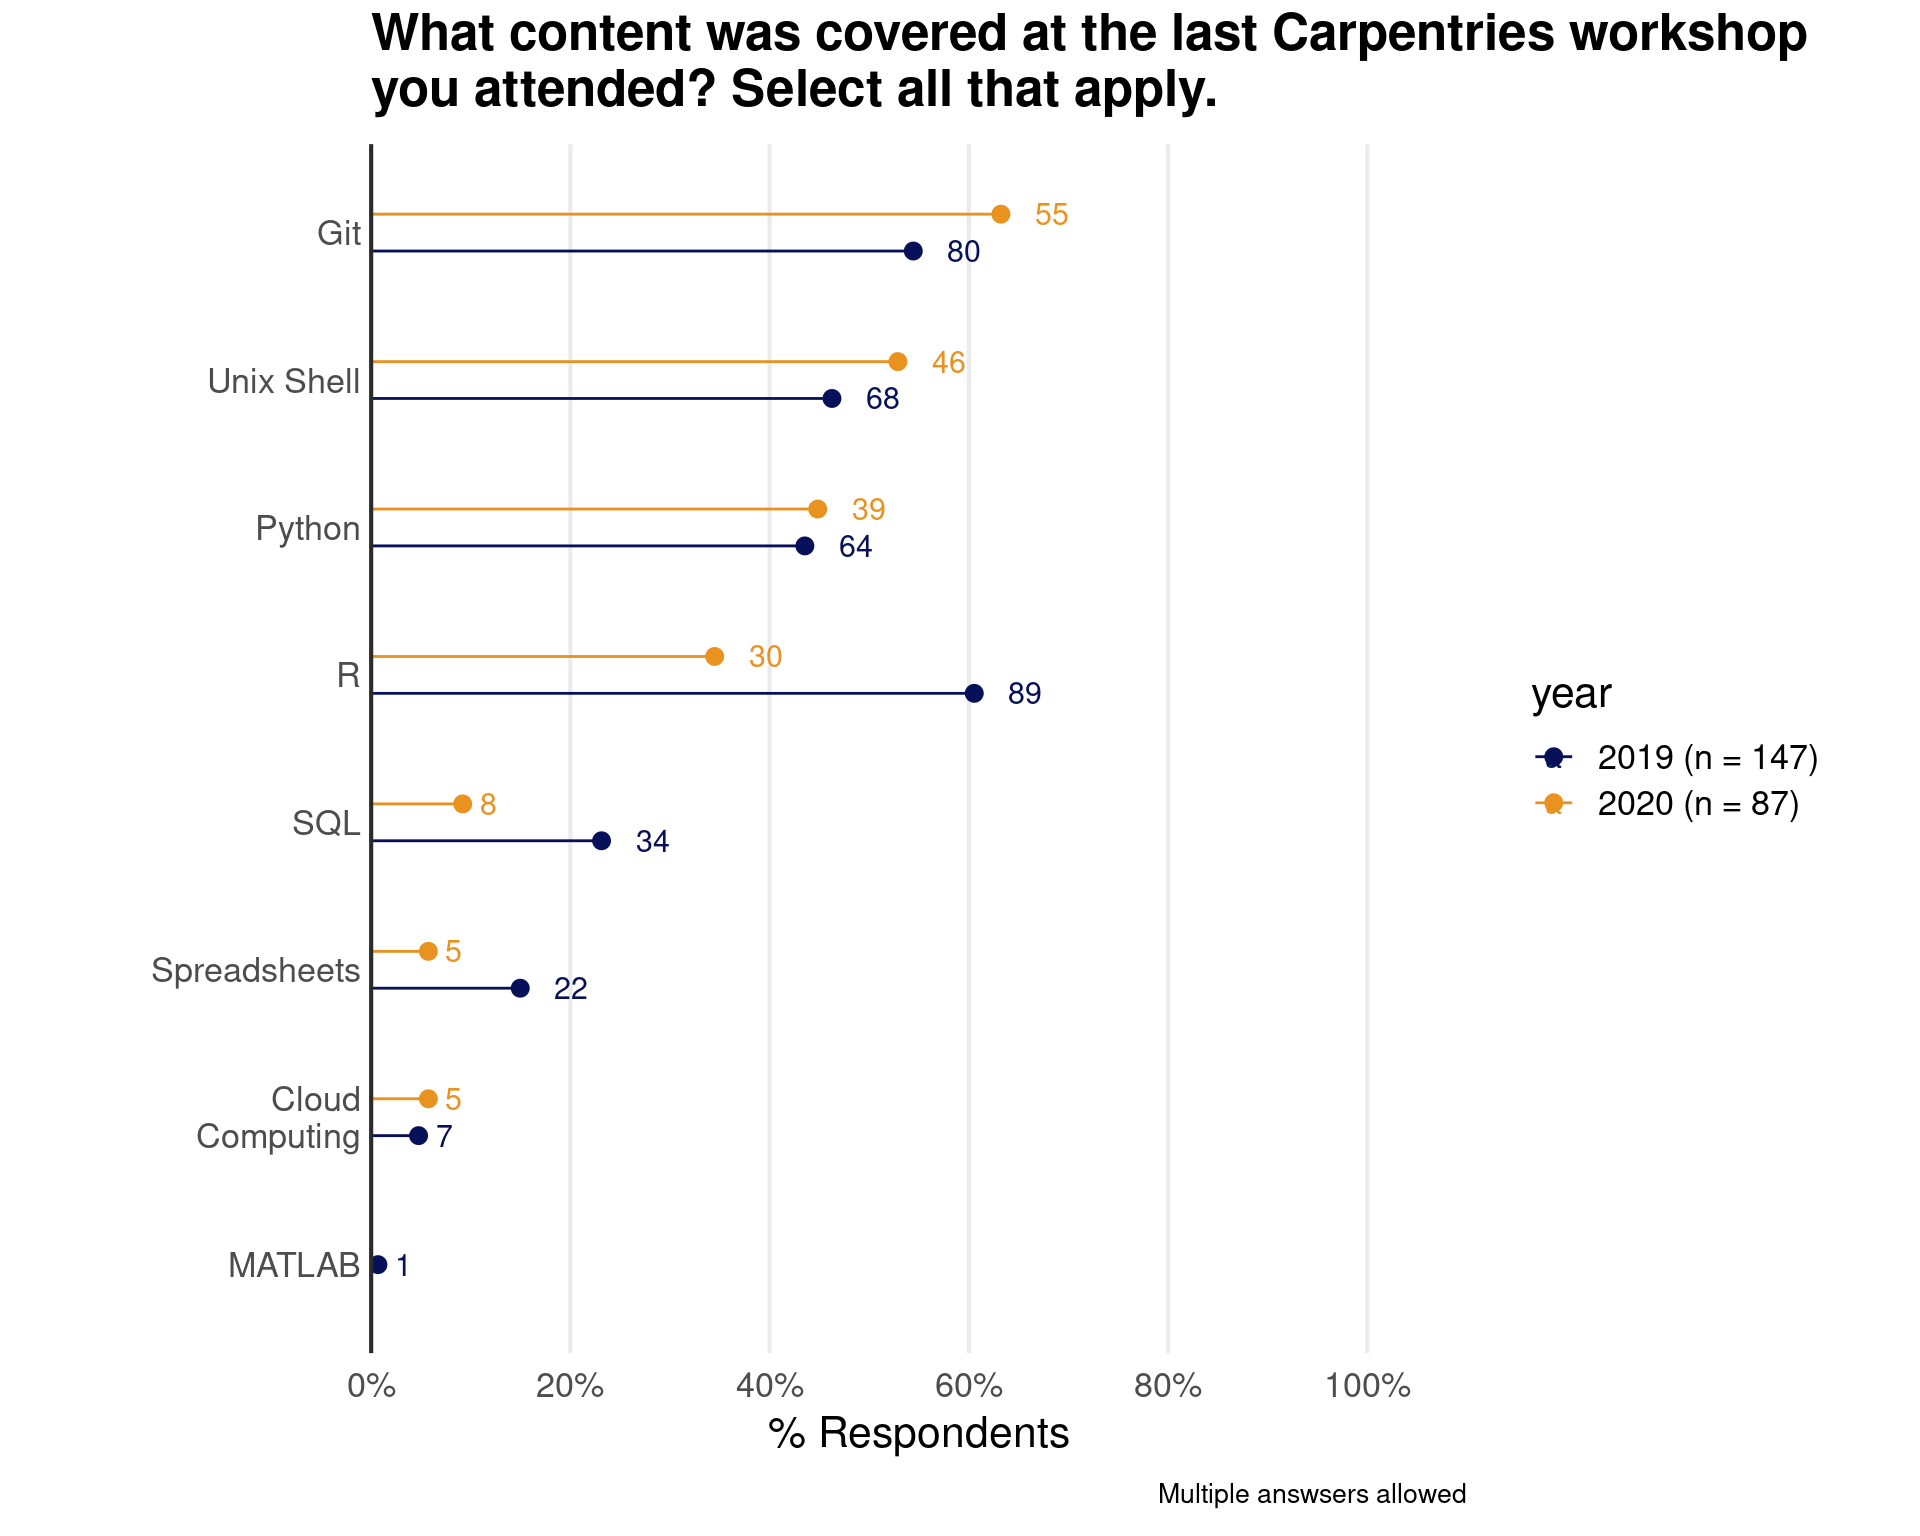
\includegraphics[width=\maxwidth]{../figures/2020-12-longterm-workshop_attended_content-1}

\hypertarget{behaviors-adopted}{%
\subsection{Behaviors Adopted}\label{behaviors-adopted}}

Long-term survey respondents reported that they were most likely to
adopt \emph{using version control to manage code} followed by
\emph{Other} behaviors.

\begin{verbatim}
## Warning: It is deprecated to specify `guide = FALSE` to remove a guide.
## Please use `guide = "none"` instead.
\end{verbatim}

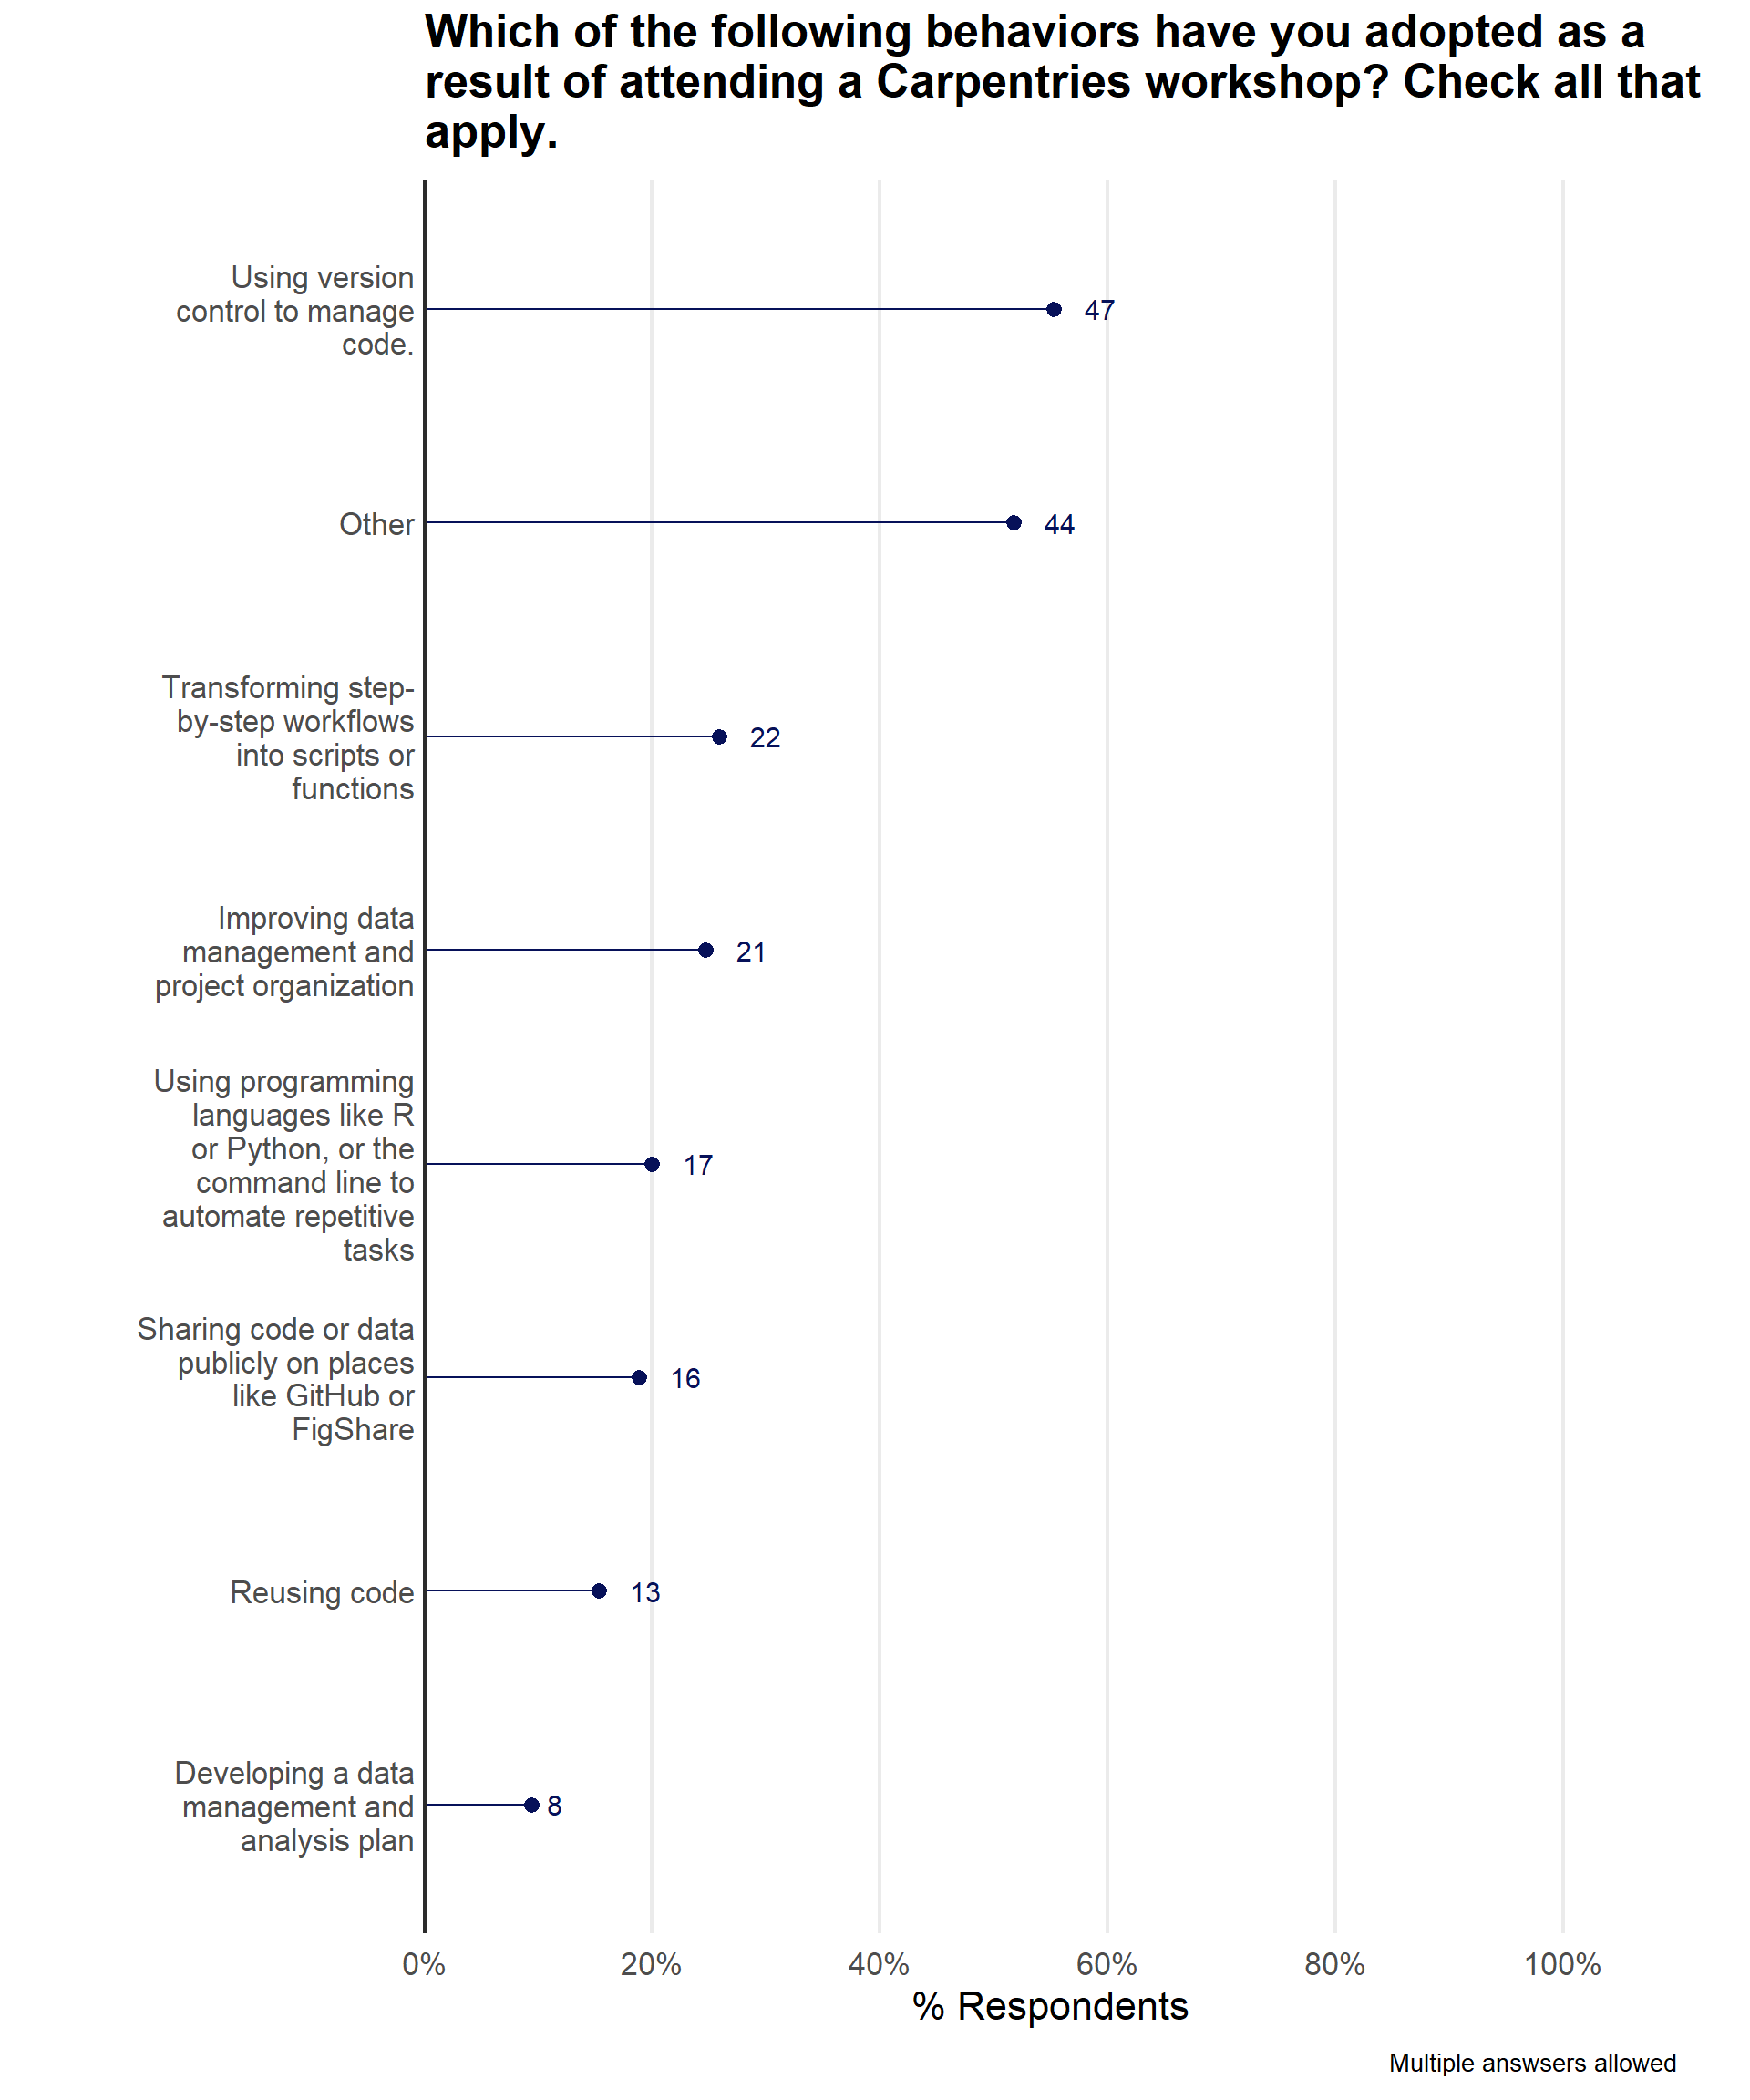
\includegraphics[width=\maxwidth]{../figures/2020-12-longterm-behavior_adopted-1}

\hypertarget{comparison-of-programming-usage-pre--and-post-carpentries-workshop}{%
\subsection{Comparison of Programming Usage Pre- and Post-Carpentries
Workshop}\label{comparison-of-programming-usage-pre--and-post-carpentries-workshop}}

Long-term survey respondents reported using programming languages,
databases, version control and/or the shell more frequently after taking
a Carpentries workshop. Of particular note is the increase in people who
now use these tools daily or weekly as well as the drastic decrease in
those reporting they don't use these tools.

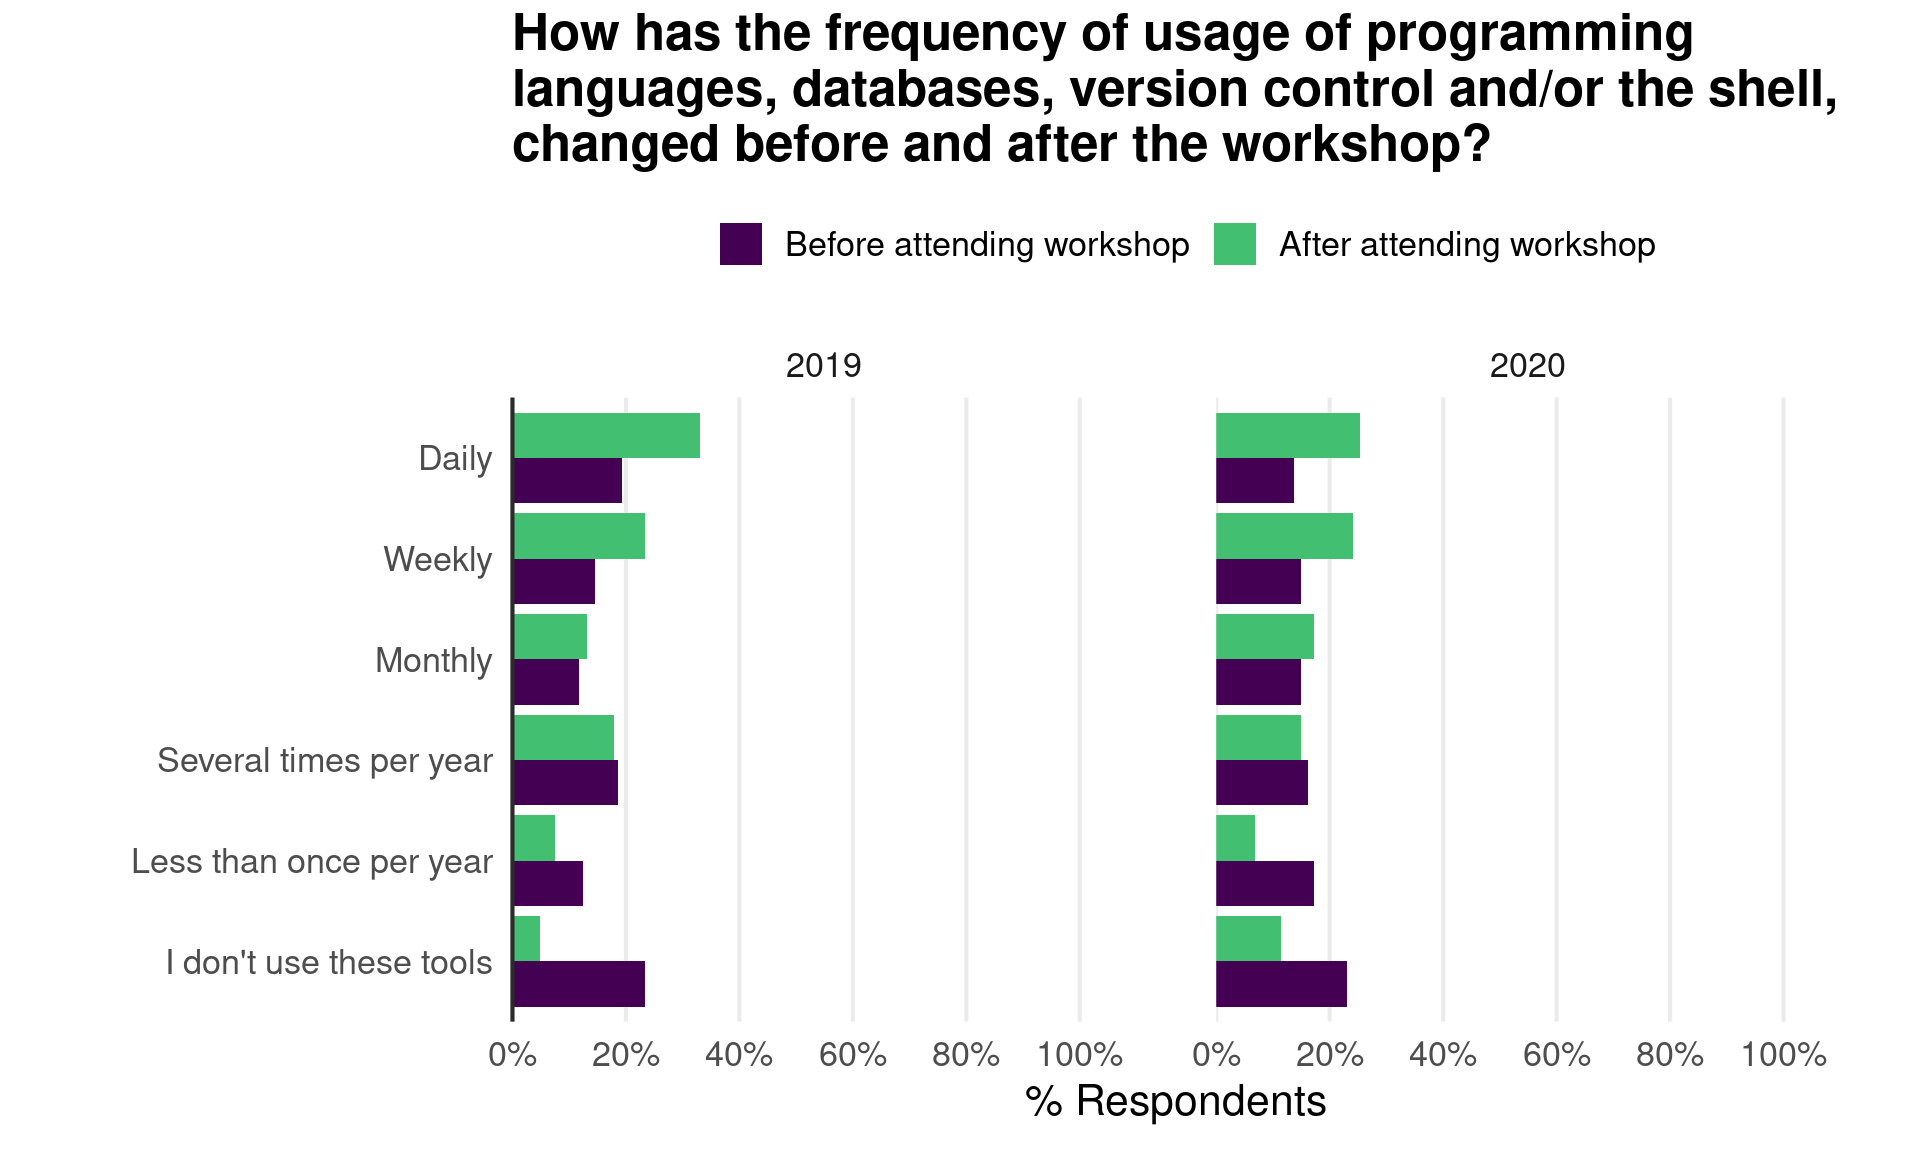
\includegraphics[width=\maxwidth]{../figures/2020-12-longterm-change_usage_frequency-1}

\hypertarget{change-in-confidence-in-tools-covered-at-workshop}{%
\subsection{Change in Confidence in Tools Covered at
Workshop}\label{change-in-confidence-in-tools-covered-at-workshop}}

The vast majority of long-term survey respondents reported that they are
more confident using tools covered in the workshop after compared to
before.

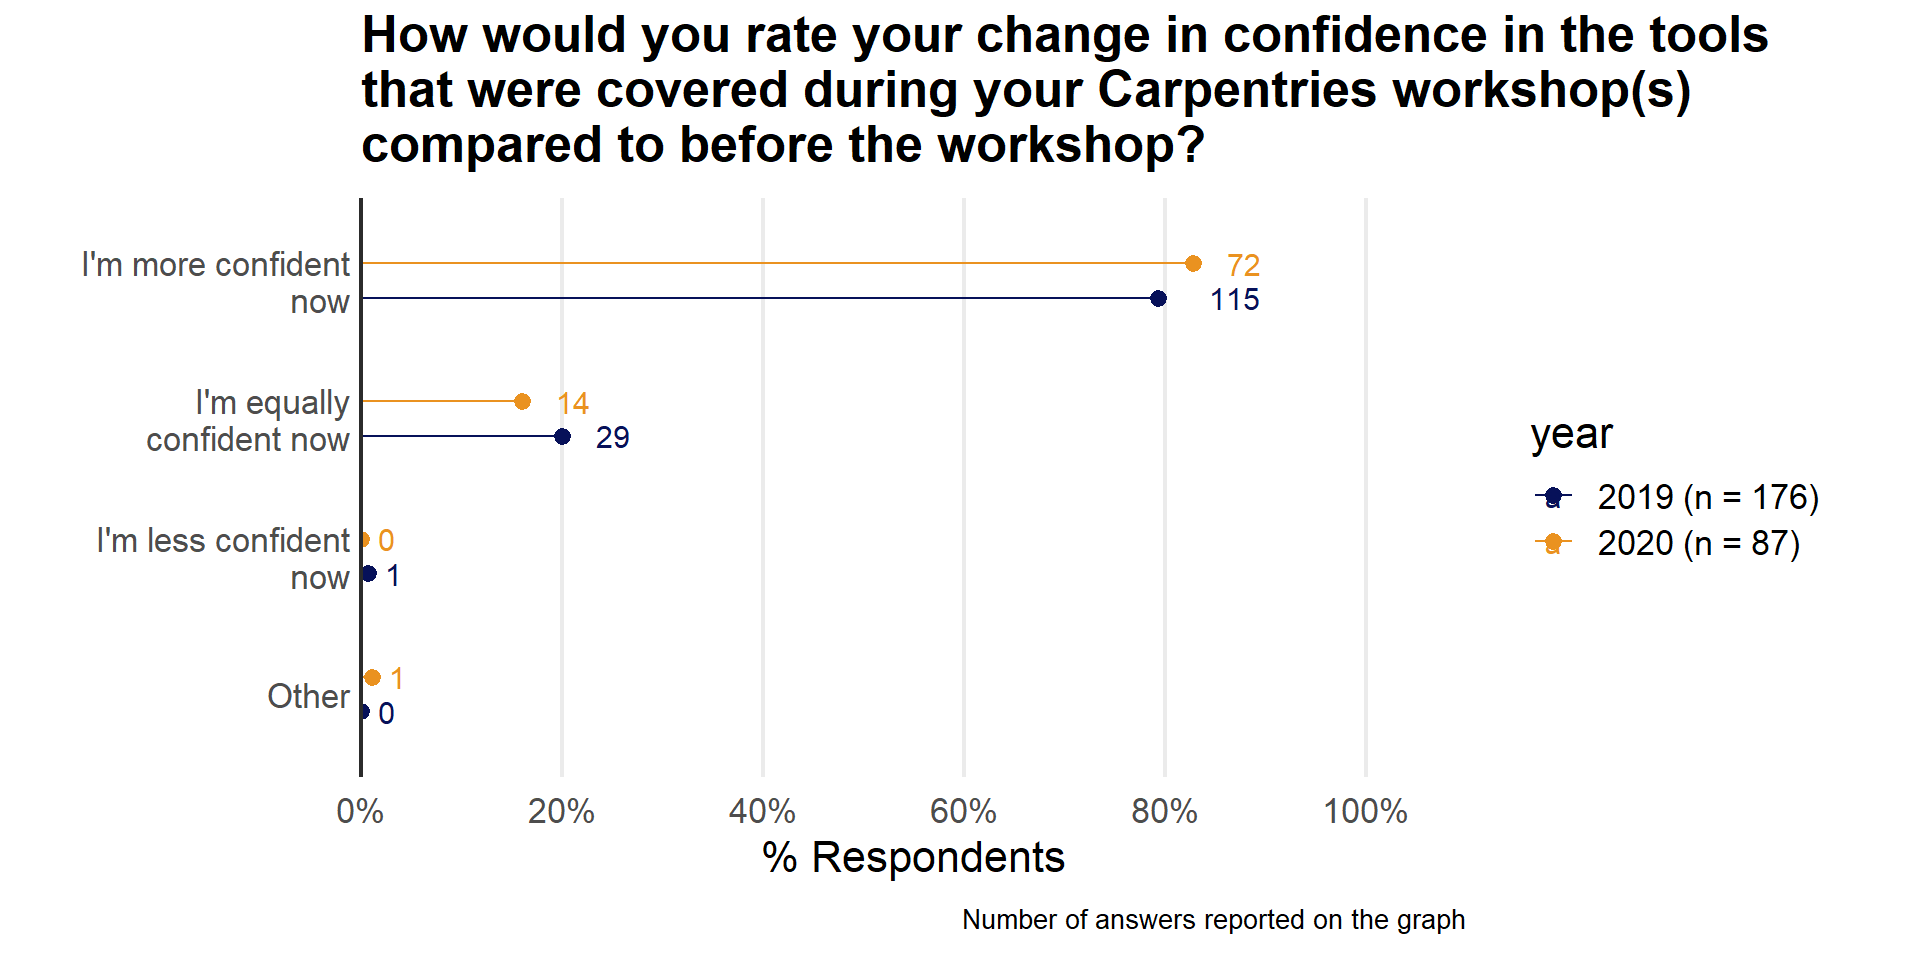
\includegraphics[width=\maxwidth]{../figures/2020-12-longterm-change_confidence-1}

\hypertarget{how-tools-help-respondents}{%
\subsection{How Tools Help
Respondents}\label{how-tools-help-respondents}}

Long-term survey respondents report that using the tools they learned in
a Carpentries workshop are improving their overall efficiency as well as
their ability to analyze and manage data.

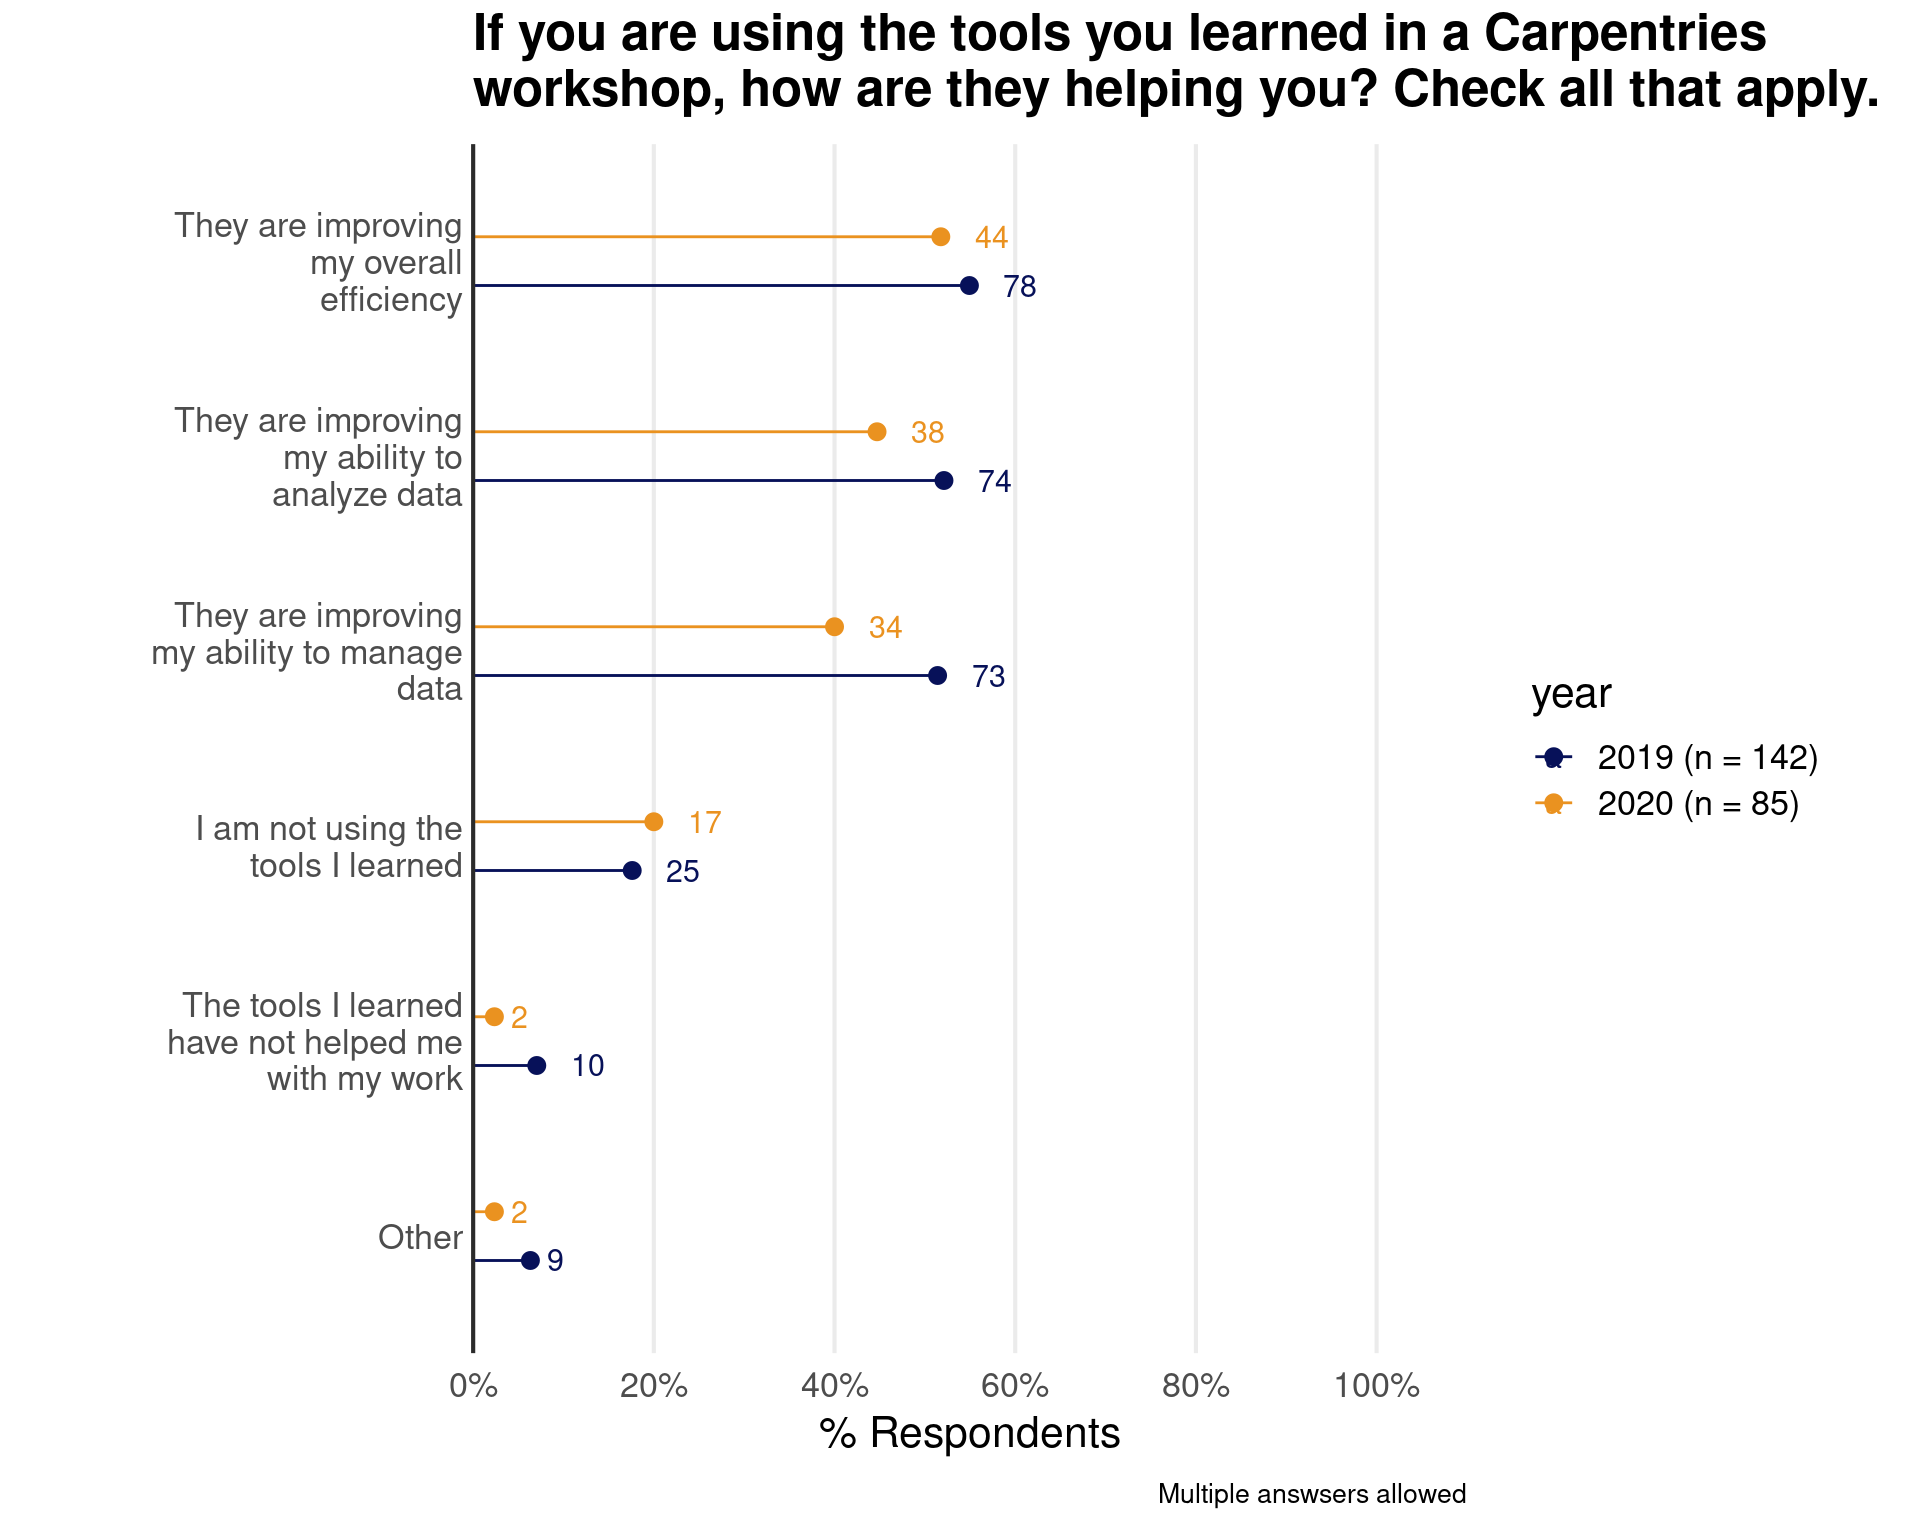
\includegraphics[width=\maxwidth]{../figures/2020-12-longterm-how_tools_help-1}

\hypertarget{carpentries-workshop-contributing-to-research}{%
\subsection{Carpentries Workshop Contributing to
Research}\label{carpentries-workshop-contributing-to-research}}

For about a quarter of long-term survey respondents, attending a
Carpentries workshop has contributed to their writing of a research
article, thesis, dissertation, or grant proposal.

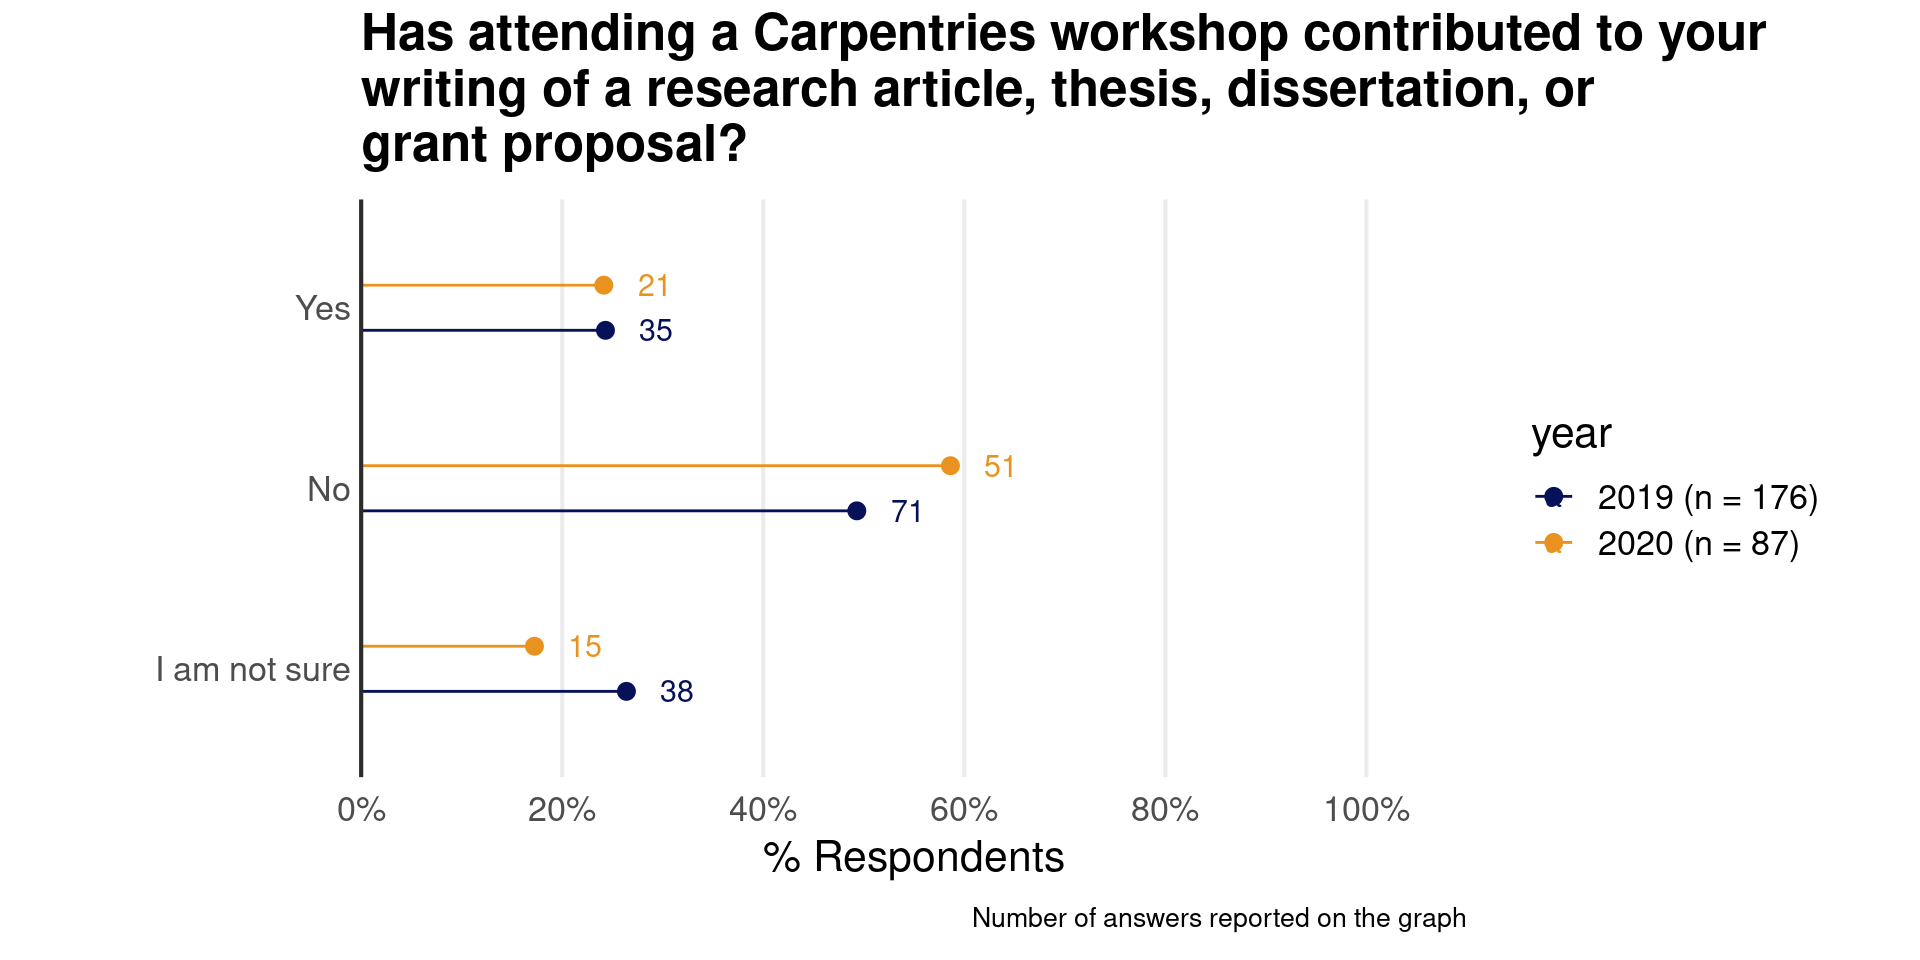
\includegraphics[width=\maxwidth]{../figures/2020-12-longterm-workshop_contributed_academics-1}

\hypertarget{potential-impact-on-respondents}{%
\subsection{Potential Impact on
Respondents}\label{potential-impact-on-respondents}}

As a result of taking a Carpentries workshop, the majority of long-term
survey respondents agree that they:

\begin{itemize}
\tightlist
\item
  have used skills learned at the workshop to advance their career;
\item
  improved their coding practices;
\item
  have gained confidence in working with data;
\item
  made their analyses more reproducible; and
\item
  been motivated to seek more knowledge about the tools learned.
\end{itemize}

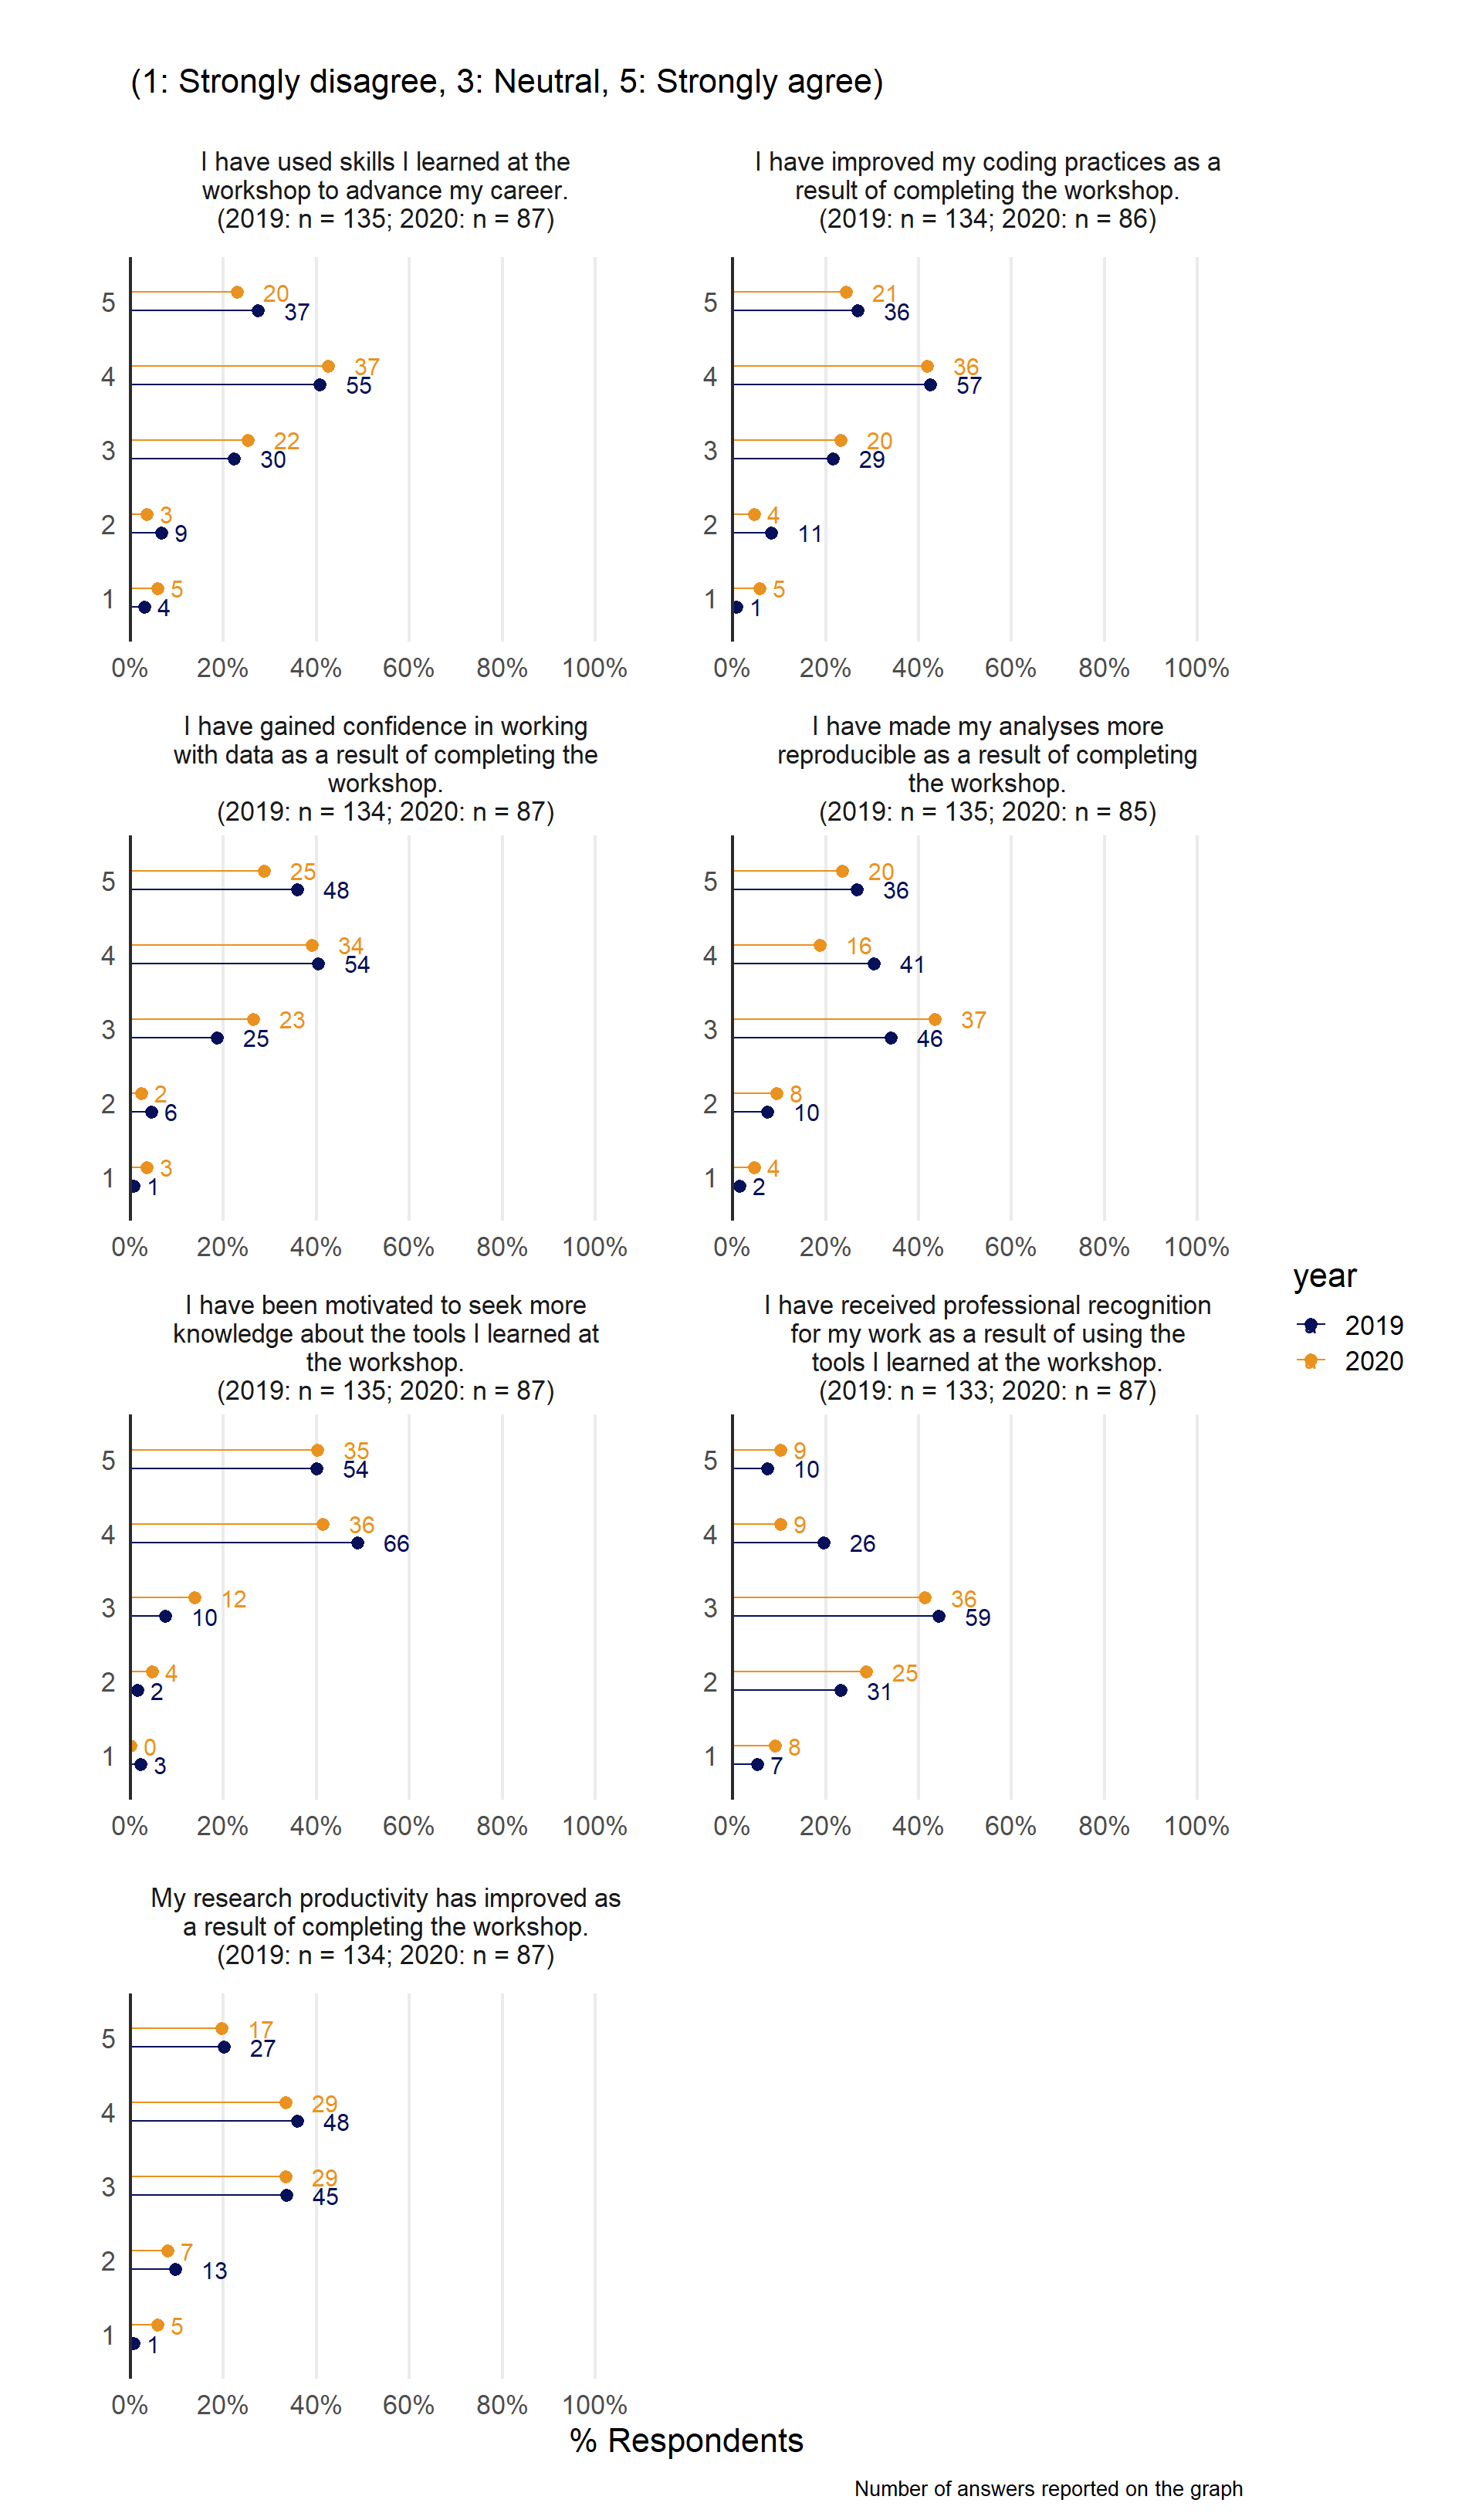
\includegraphics[width=\maxwidth]{../figures/2020-12-longterm-workshop_impact-1}

\hypertarget{involvement-in-carpentries-community-post-workshop}{%
\subsection{Involvement in Carpentries Community
Post-Workshop}\label{involvement-in-carpentries-community-post-workshop}}

Following the workshop, the majority of long-term survey respondents
have subscribed to the Carpentries newsletter. Smaller numbers of
respondents have gotten involved in the Carpentries community in other
ways, include attending a community discussion, engaging on Twitter, and
becoming a workshop helper.

\begin{verbatim}
## Warning: It is deprecated to specify `guide = FALSE` to remove a guide.
## Please use `guide = "none"` instead.
\end{verbatim}

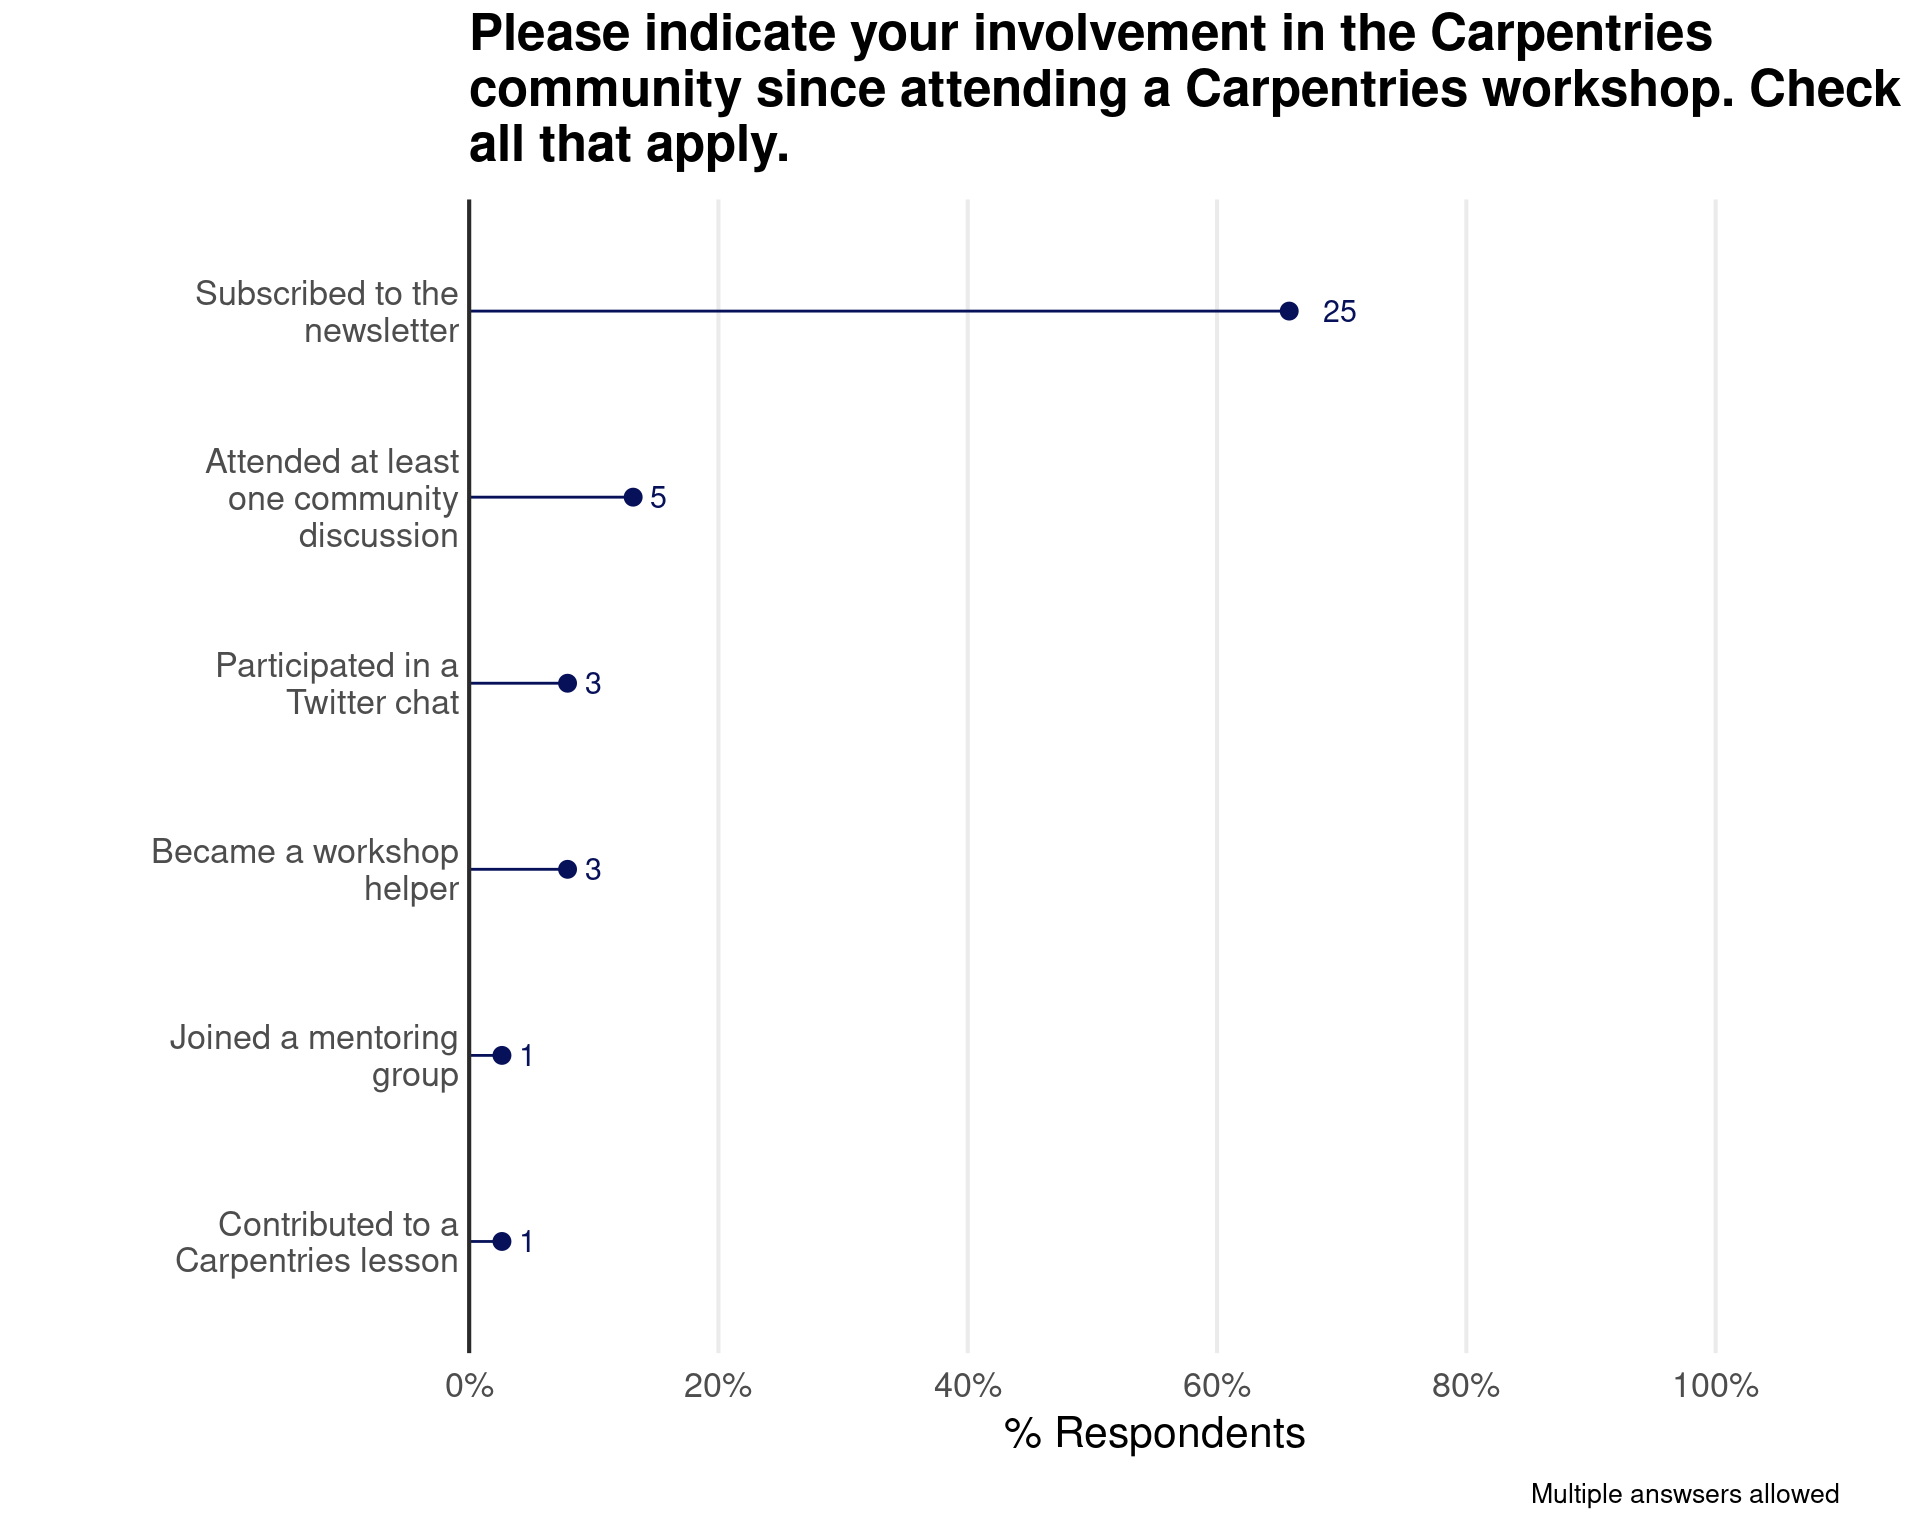
\includegraphics[width=\maxwidth]{../figures/2020-12-longterm-community_involvement-1}

\hypertarget{respondents-participating-in-learning-activities}{%
\subsection{Respondents Participating in Learning
Activities}\label{respondents-participating-in-learning-activities}}

Many long-term survey respondents have continued learning after taking a
Carpentries workshop. The most common ways they continued learning were
by using both Carpentries and non-Carpentries self-guided lesson
material. Smaller numbers participated in additional courses (e.g.,
online short courses, in-person short courses, or semester-long
courses).

\begin{verbatim}
## Warning: It is deprecated to specify `guide = FALSE` to remove a guide.
## Please use `guide = "none"` instead.
\end{verbatim}

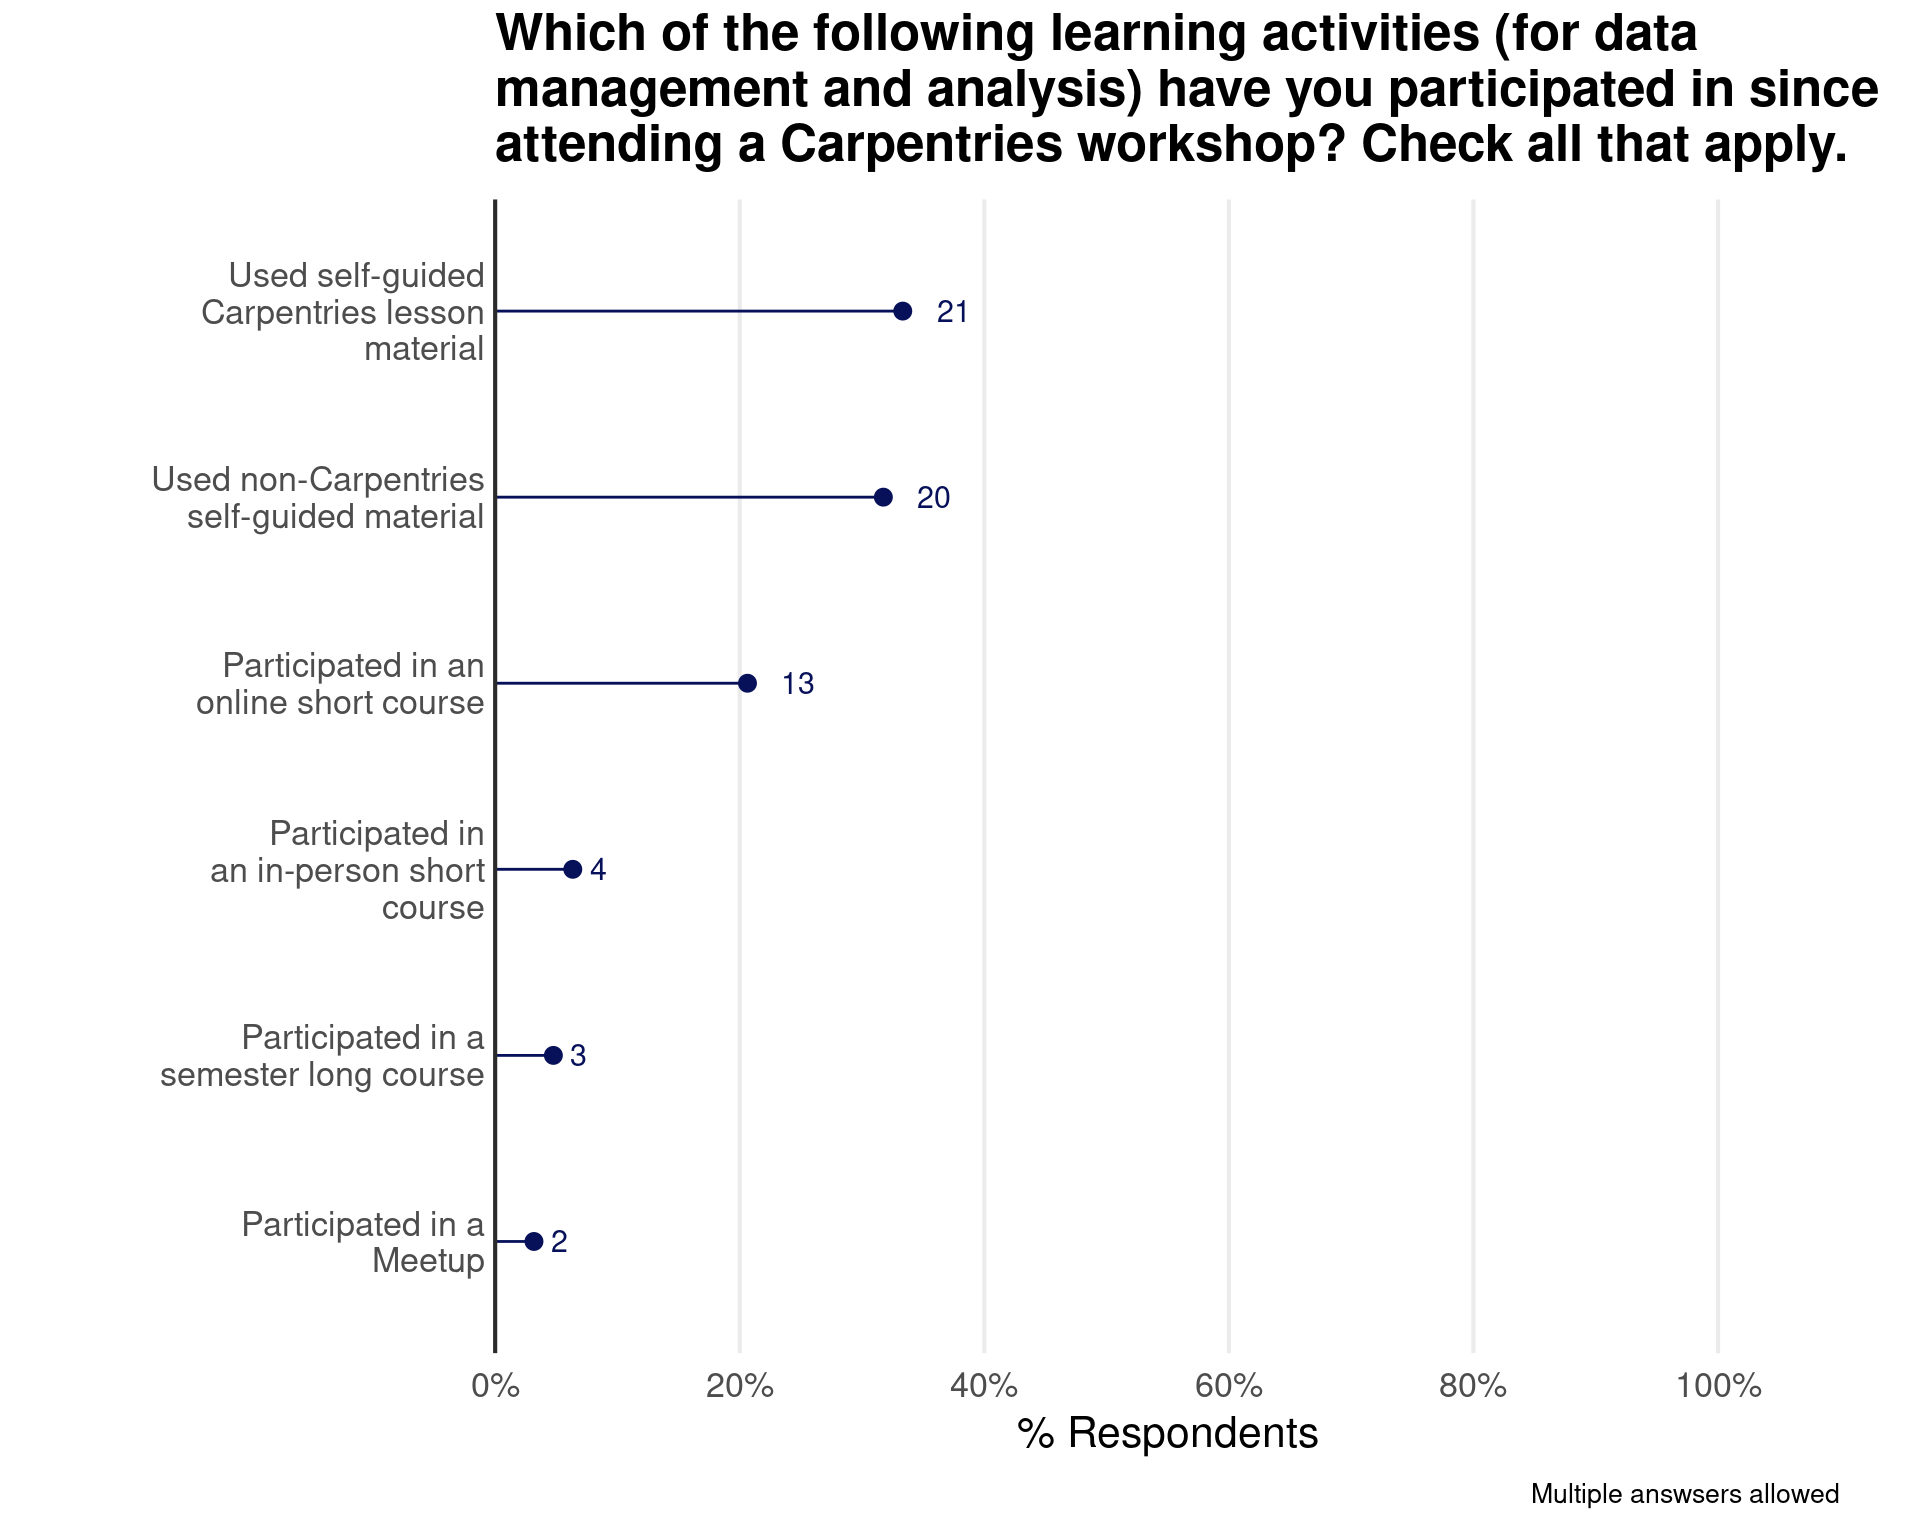
\includegraphics[width=\maxwidth]{../figures/2020-12-longterm-other_activities-1}

\hypertarget{respondents-who-recommended-a-carpentries-workshop}{%
\subsection{Respondents Who Recommended a Carpentries
Workshop}\label{respondents-who-recommended-a-carpentries-workshop}}

The vast majority of long-term survey respondents reported that they
have recommended a Carpentries workshop to a friend or colleague.

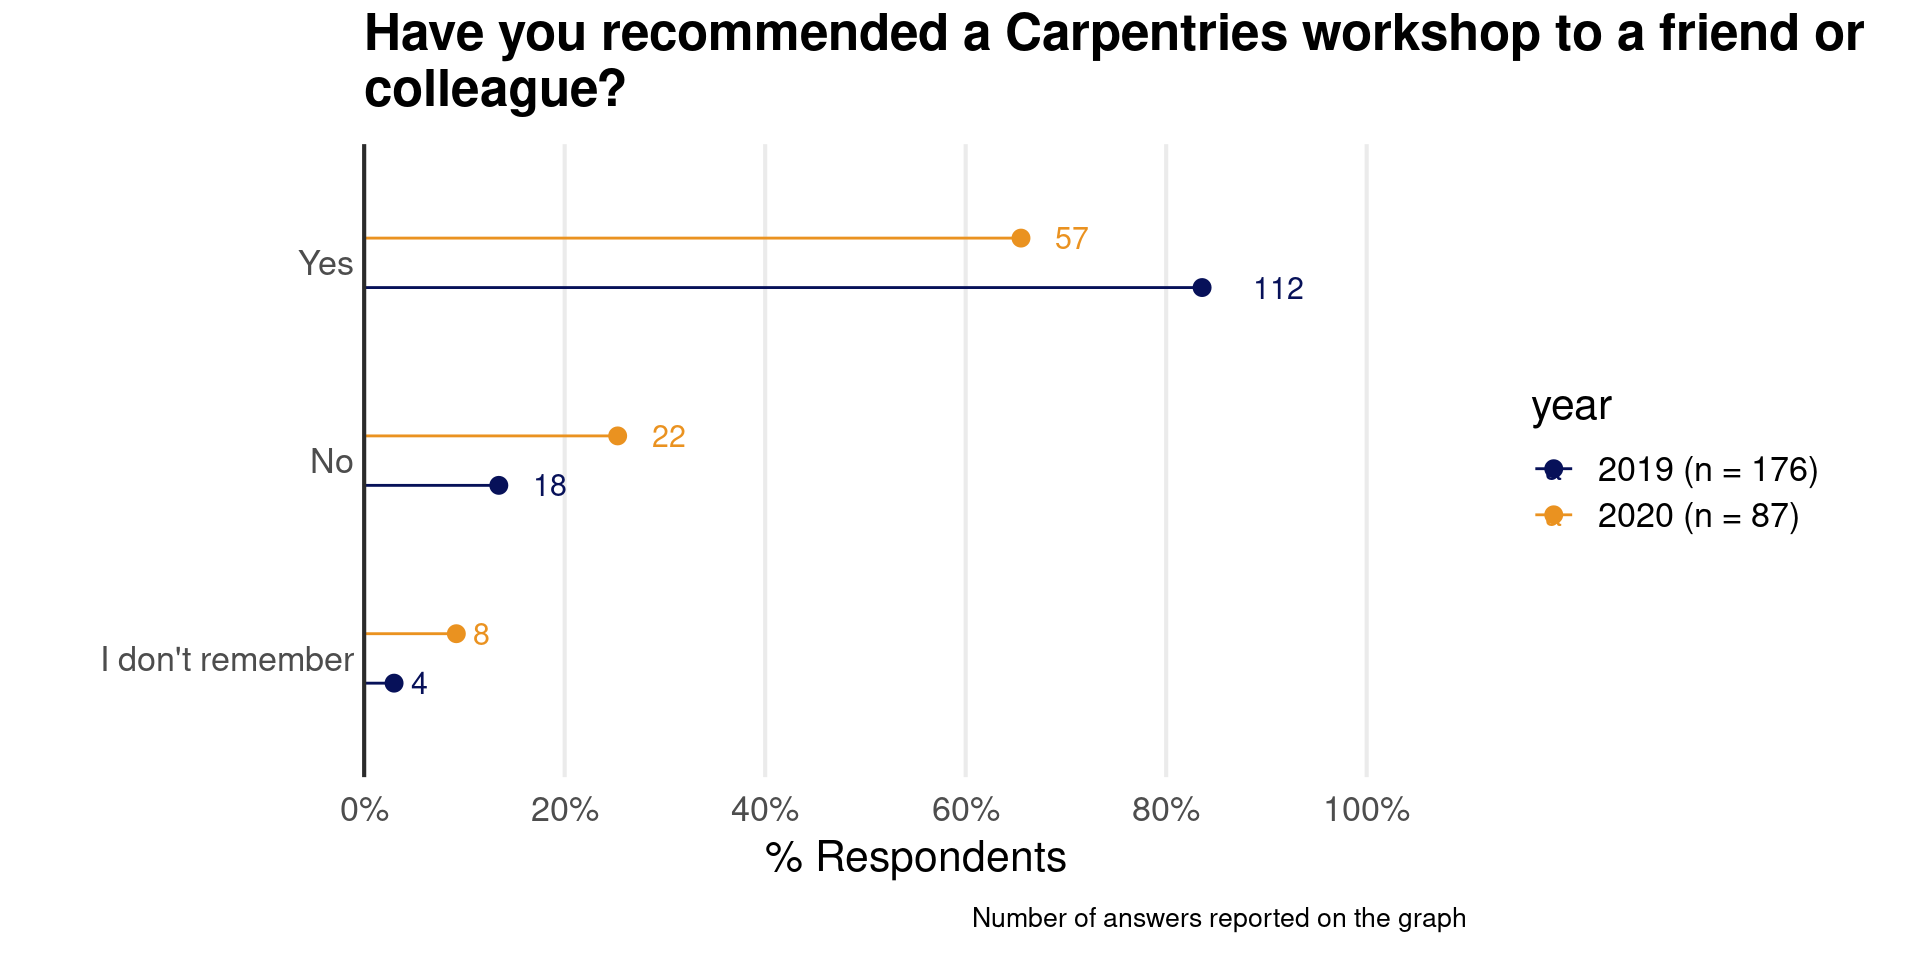
\includegraphics[width=\maxwidth]{../figures/2020-12-longterm-has_recommended-1}

\hypertarget{recommendation-and-net-promoter-scores}{%
\subsection{Recommendation and Net Promoter
Scores}\label{recommendation-and-net-promoter-scores}}

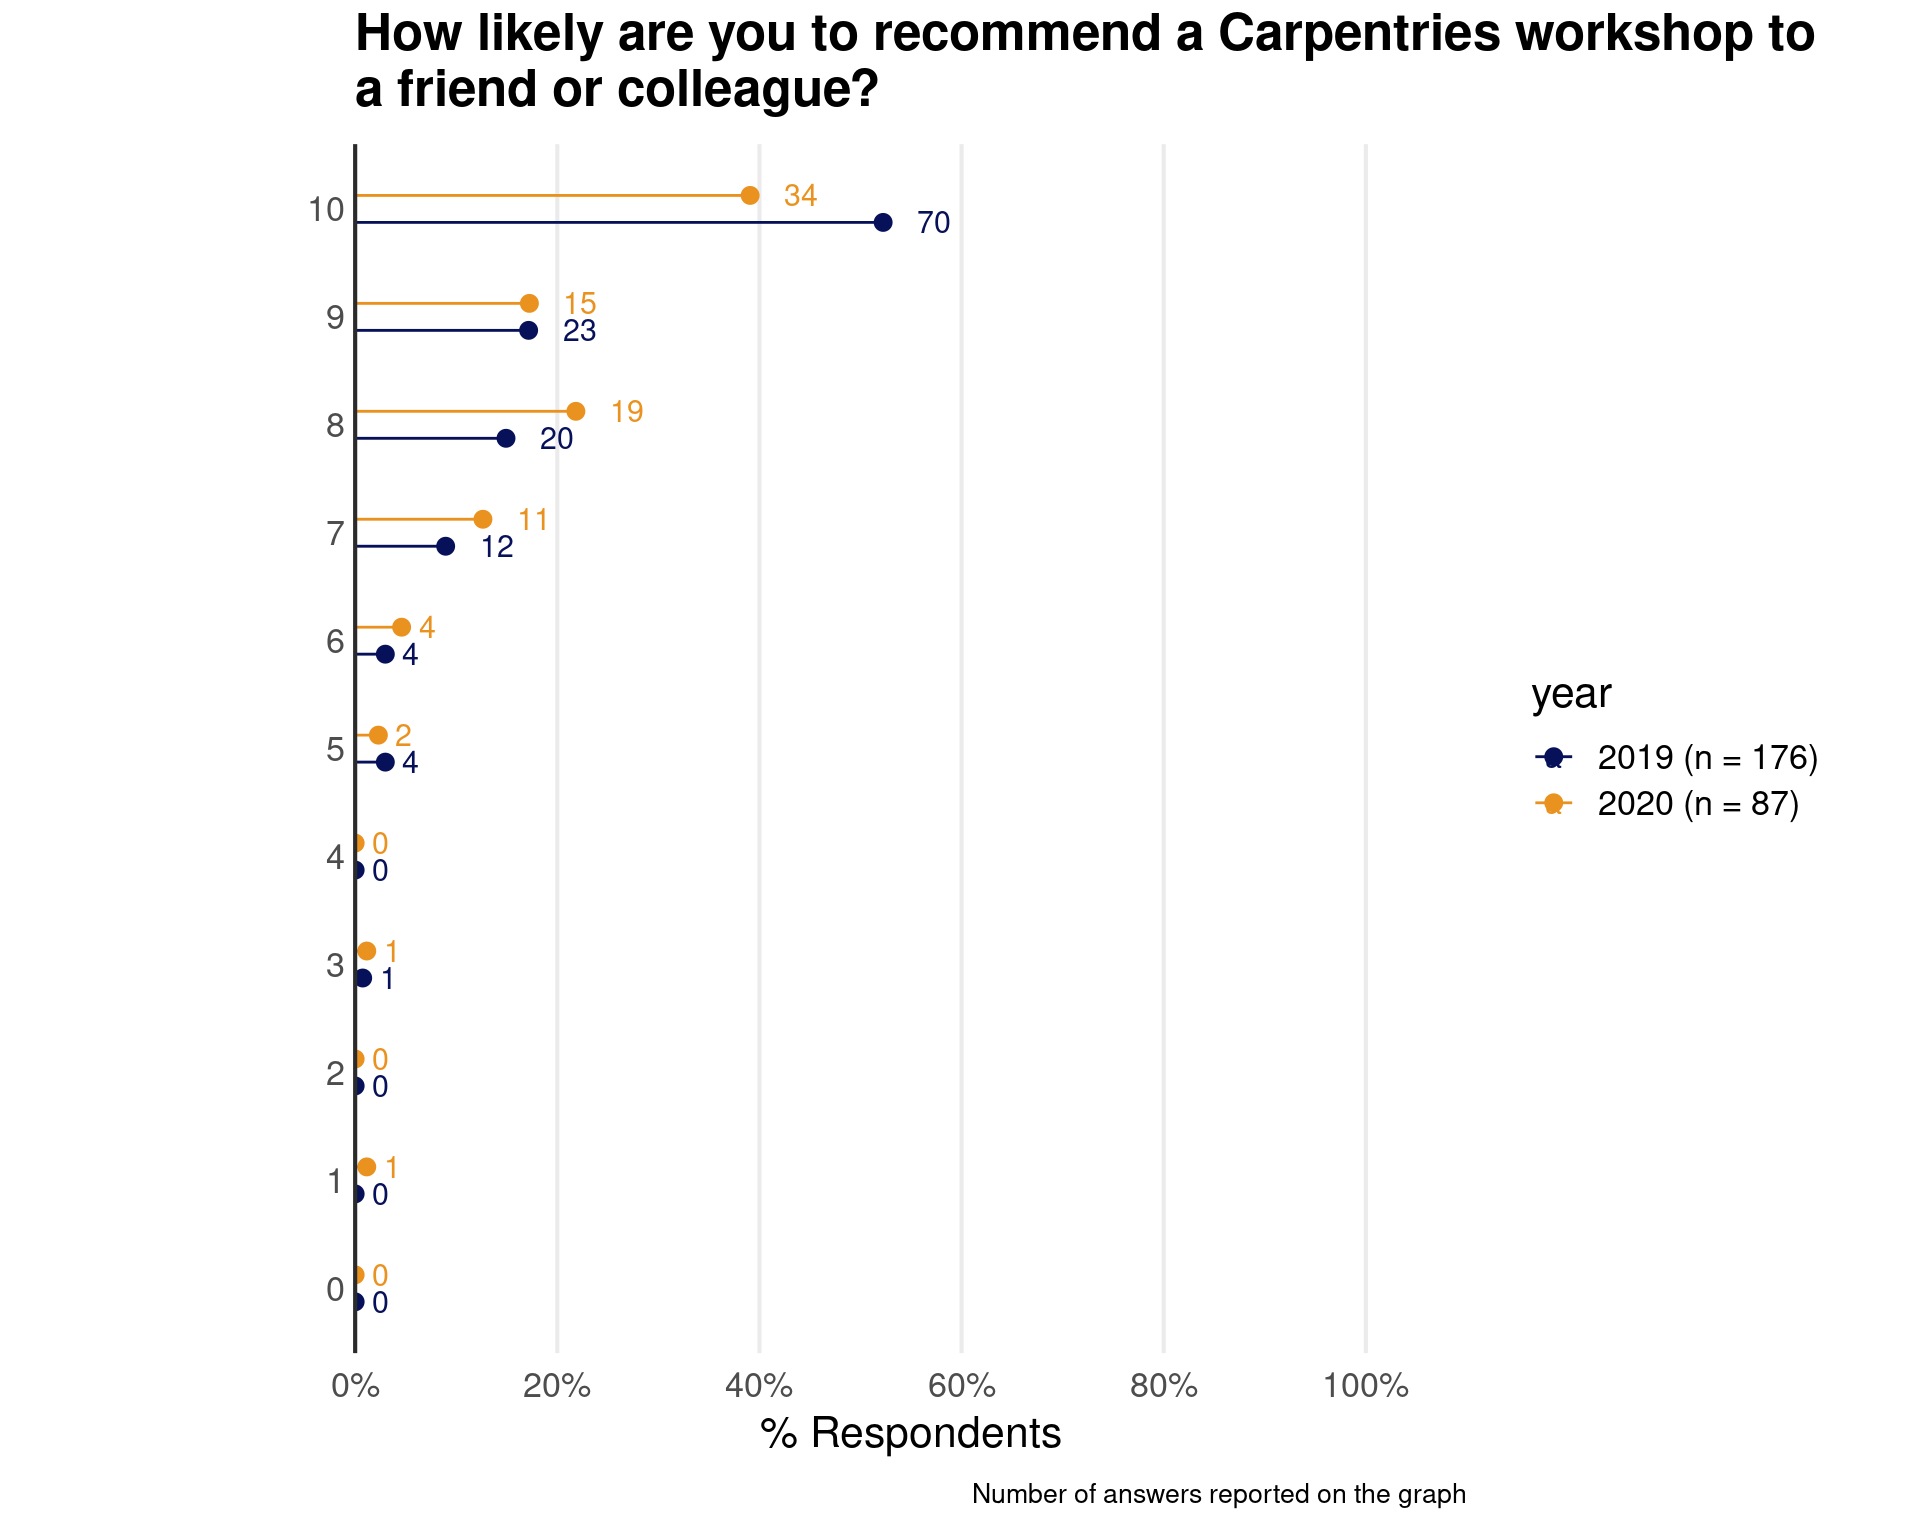
\includegraphics[width=\maxwidth]{../figures/2020-12-longterm-recommendation_score-1}

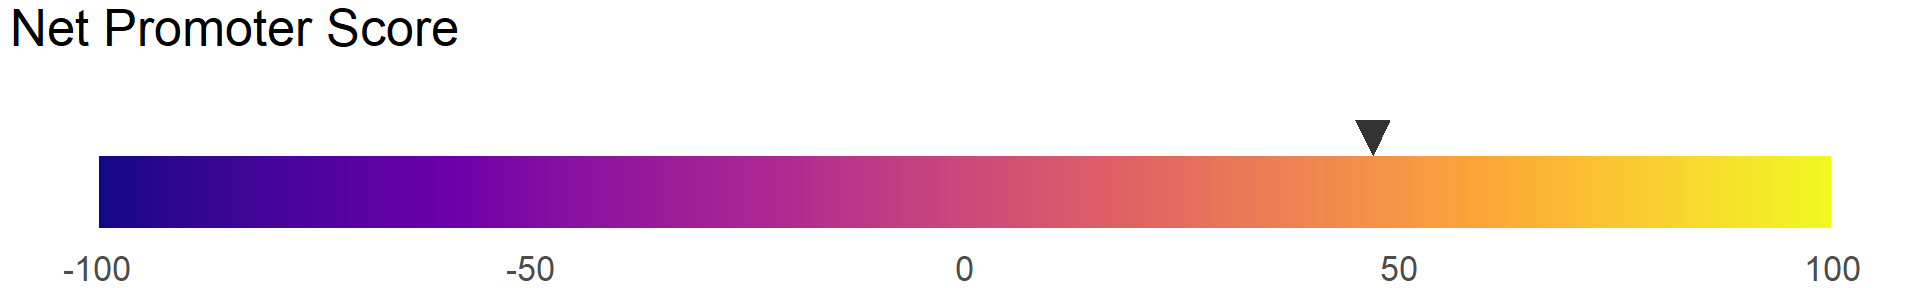
\includegraphics[width=\maxwidth]{../figures/2020-12-longterm-nps-1}

The \href{https://en.wikipedia.org/wiki/Net_Promoter}{Net Promoter
Score} (NPS) for our workshops according to the long-term survey is 47.
The NPS varies between -100 and +100. It is calculated by substracting
the percentage of respondents who are considered ``Promoters'' (rating
of 9 or 10) and the percentage of respondents who are considered
``Detractors'' (rating equal or below 6). A positive NPS is deemed good,
a NPS above 50 is deemed excellent, and an NPS above 70 is exceptional.

\hypertarget{respondents-gender-identity}{%
\subsection{Respondents' Gender
Identity}\label{respondents-gender-identity}}

Note: Gender identity responses apply to U.S. survey respondents only.

A higher percentage of US-based long-term survey respondents are females
compared with males or those who are gender variant/non-conforming.

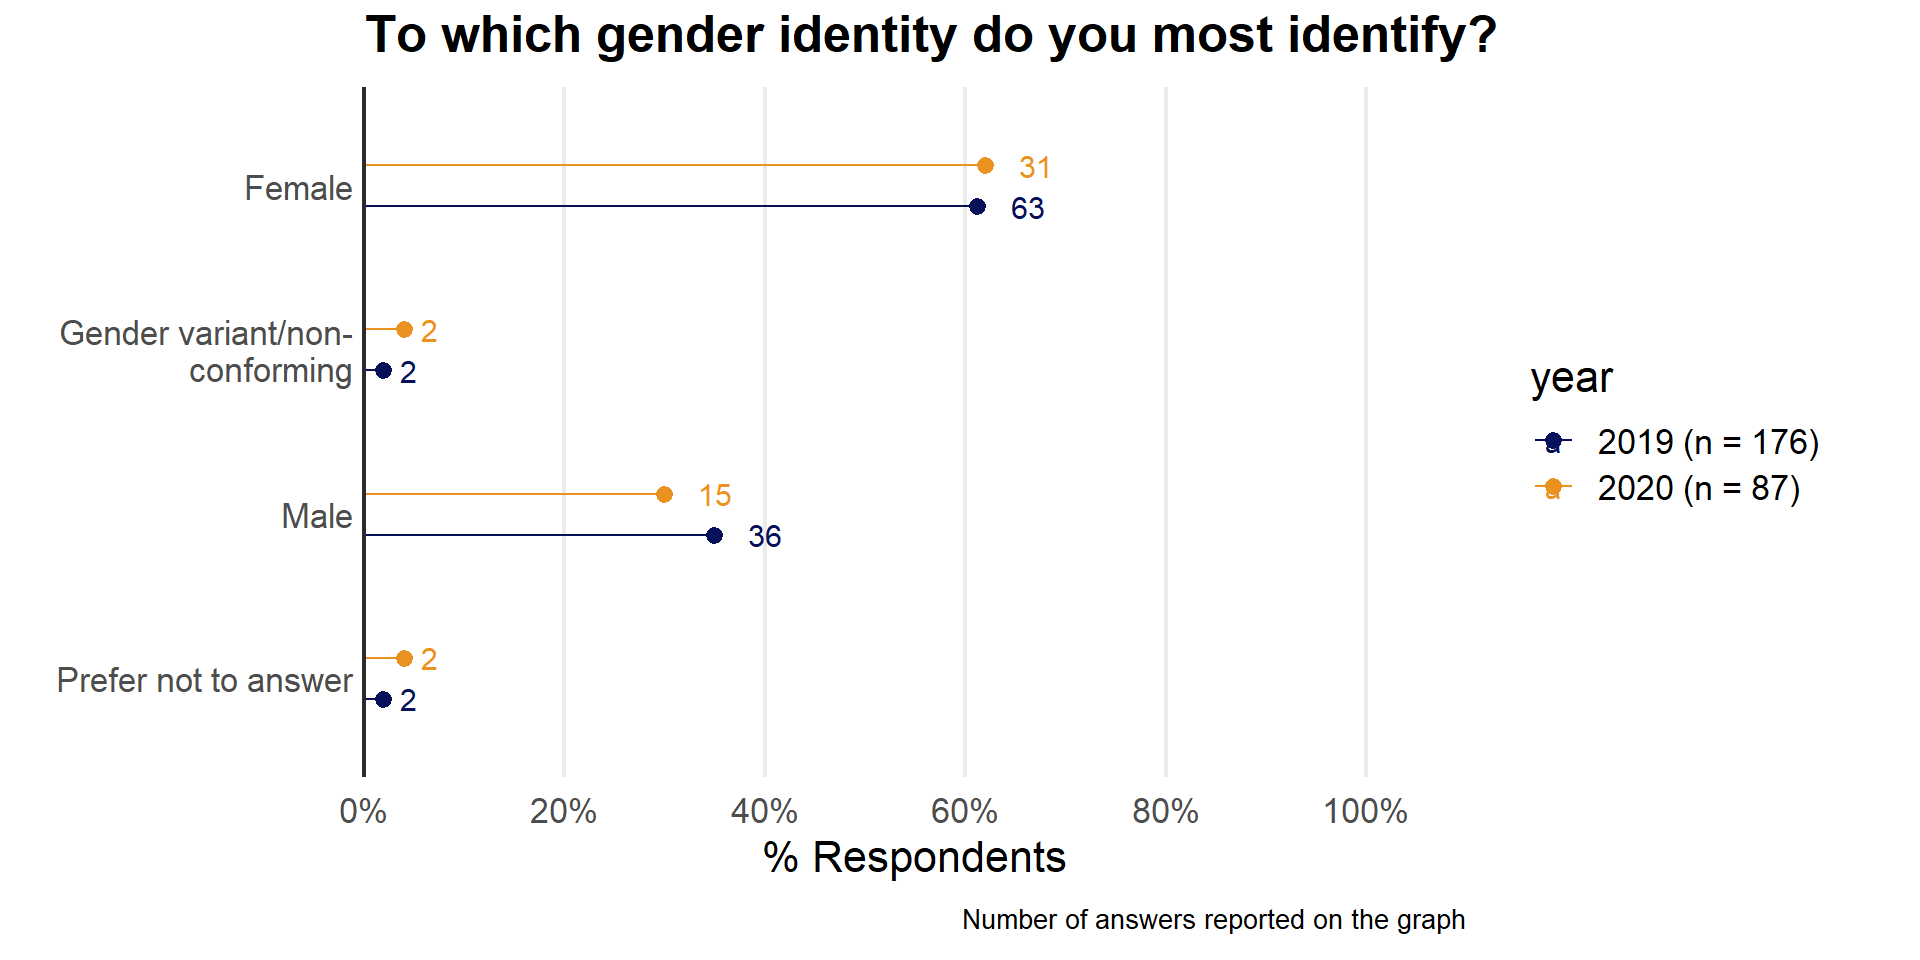
\includegraphics[width=\maxwidth]{../figures/2020-12-longterm-demographics_gender-1}

\hypertarget{respondents-racialethnic-identity}{%
\subsection{Respondents' Racial/Ethnic
Identity}\label{respondents-racialethnic-identity}}

Note: Racial/ethnic identity responses apply to U.S. survey respondents
only.

The highest percentage of US-based long-term survey respondents
self-identify as White with smaller percentages identifying as Hispanic
or Latino/a, Black or African American, and Asian.

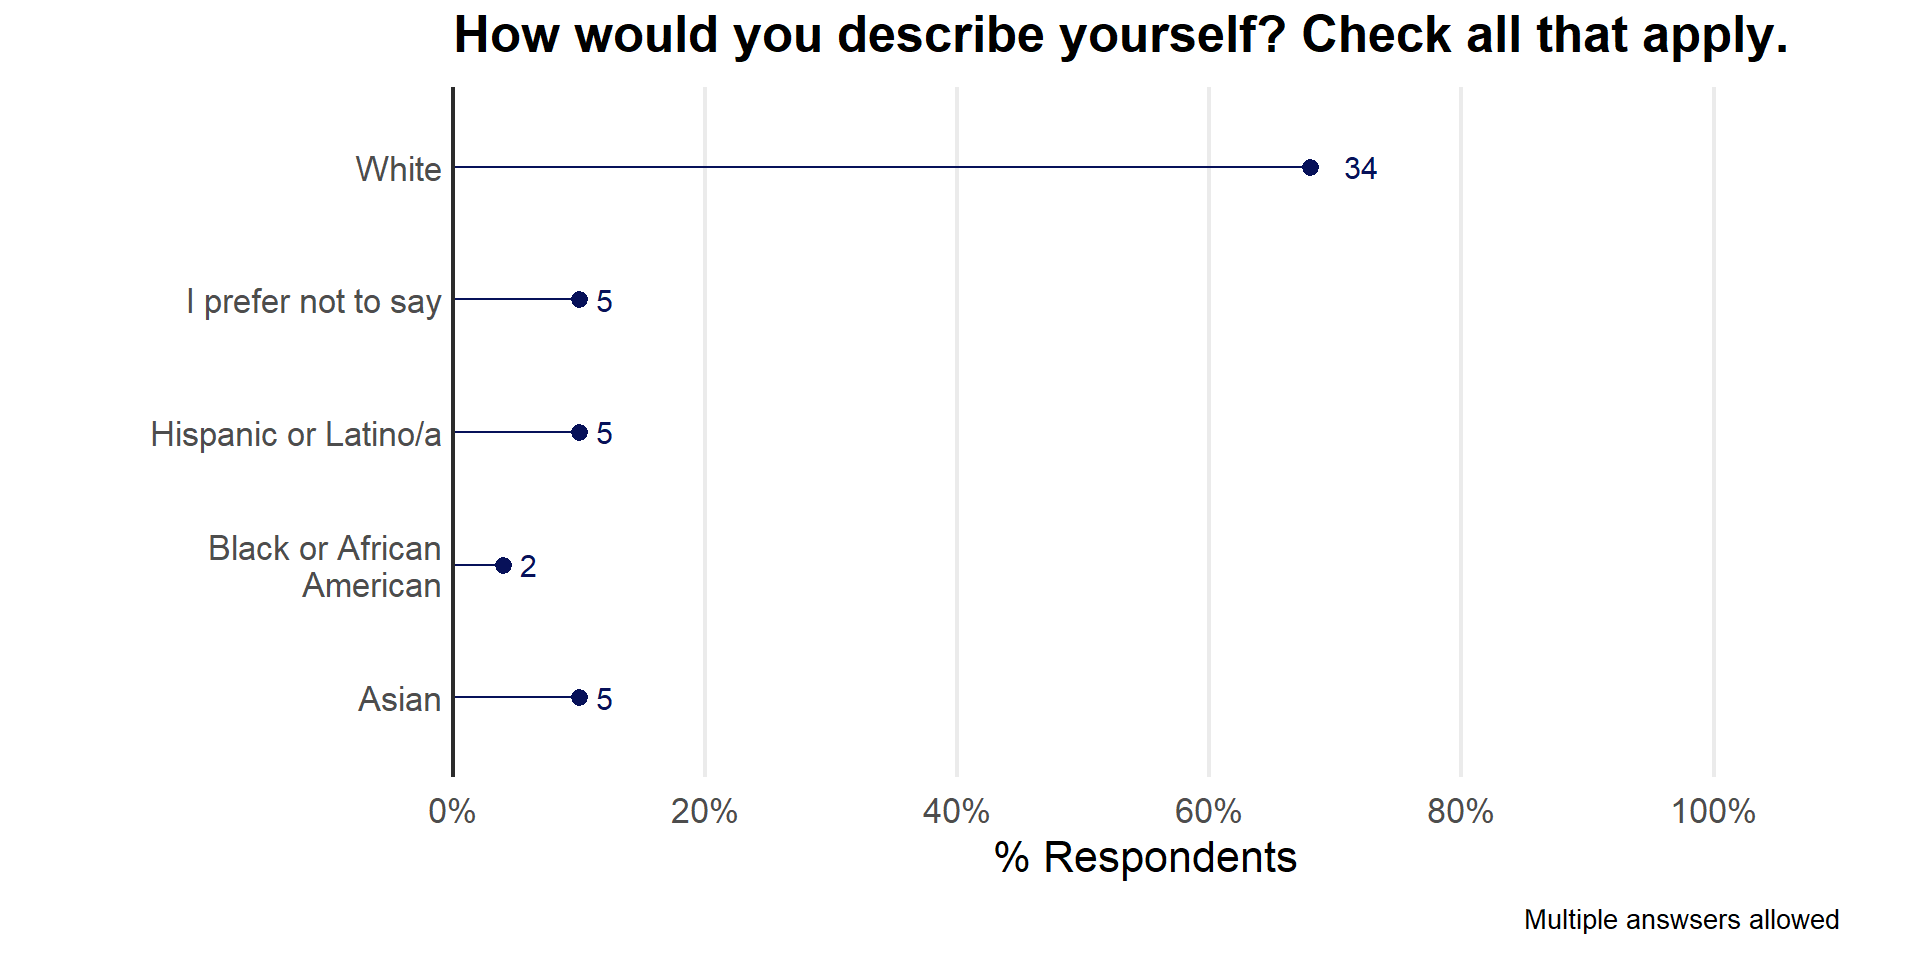
\includegraphics[width=\maxwidth]{../figures/2020-12-longterm-demographics_ethnicity-1}

\begin{table}
\centering
\begin{tabular}{l>{\raggedright\arraybackslash}p{7cm}}
\toprule
Label on Plot & Description in Survey\\
\midrule
I prefer not to say & I prefer not to say\\
White & White (Having origins in any of the original peoples of Europe, the Middle East, or North Africa.)\\
Pacific Islander & Native Hawaiian or Other Pacific Islander (Having origins in any of the original peoples of Hawaii, Guam, Samoa, or other Pacific Islands.)\\
Hispanic or Latino/a & Hispanic or Latino(a) (A person of Spanish-speaking origin or ancestry and/or Latin American origin or ancestry – includes Portuguese and Brazilians.)\\
Black or African American & Black or African American (Having origins in any of the Black racial groups of Africa – includes Caribbean Islanders and others of African origin.)\\
\addlinespace
Asian & Asian (Having origins in any of the original peoples of the Far East, Southeast Asia, or the Indian subcontinent including, for example, Cambodia, China, India, Japan, Korea, Malaysia, Pakistan, Indonesia, the Philippine Islands, Thailand, and Vietnam.)\\
American Indian or Alaska Native & American Indian or Alaska Native (Having origins in any of the original peoples of North and South America (including Central America), and who maintains a tribal affiliation or community attachment.)\\
\bottomrule
\end{tabular}
\end{table}

\end{document}
